\documentclass{memoria}
\usepackage{amsmath}
\usepackage{graphicx} 
\usepackage{float}
\usepackage{caption,subcaption}
\begin{document}

\portada{Informe de laboratorio 1 de Algoritmos Numéricos: Métodos Numéricos}{Vicente Rivera}{Profesor: Óscar Rojas Díaz.}{\today}

\indices

\capitulo{Introducción}

Los algoritmos numéricos son una manera de transformar un problema matemático y resolverlo en base a operaciones numéricas. La importancia de esto es que permite la implementación computacional para obtener aproximaciones de diversos problemas.

No todos los métodos resuelven problemas en tiempos iguales, así como también no todos alcanzan la solución con la misma precisión. Al existir una infinita cantidad de problemas que pueden tener complejidad tal que no se pueda resolver en tiempo polinomial en función de su entrada, surge la necesidad de determinar cuál método puede adecuarse mejor que otros. Un método puede decirse mejor que otro para cierto problema en base a su capacidad de resolverlo bajo un estándar de eficiencia y eficacia.

Por ende, el objetivo de este informe es poner a prueba métodos numéricos sobre funciones no lineales y sistemas de ecuaciones, y compararlos en base a criterios de eficiencia y eficacia.

En el capítulo 2 se presentan las funciones no lineales y criterios de medición. Los métodos aplicados serán Bisección, Secante, Regula Falsi, Punto fijo (incluyendo Aitken y Steffensen), y Newton Raphson. Además, se incluye un problema de funciones multivariables para el método Newton Multivariable.

Luego, se muestran los resultados en gráficos de convergencia y error, junto con un resumen tabulado de los datos obtenidos. El siguiente capítulo 

En el capítulo 5, 6 y 7 se realiza el mismo procedimiento para sistemas de ecuaciones. Los métodos a comparar son: Gauss-Jacobi, Gauss-Seidel, Factorización LU, QR y Cholesky.


\capitulo{Análisis de Métodos No Lineales}
En este capítulo se trabajará con los métodos antes mencionados para la aproximación de las raíces de las siguientes funciones no lineales:


\begin{enumerate}
\item $f_{1}(x)=2x - 2^{-x}$
\item $f_{2}(x)=x^{3}-7x^{2}+14x-2$
\end{enumerate}

También, se presenta el siguiente sistema de ecuaciones con funciones multivariable para resolver utilizando el método de Newton Multivariable

{\centering

F_{1}(x_{1}, x_{2}) = \begin{cases}
  x_{1}^{2} - 10x_{2} + x_{2}^{2}+8 = 0\\
  x_{1}x_{2}^{2} - x_{1} - 10x_{2}+8 = 0\\
  X_{(0)} = (0,0)^{T}\\
\end{cases}

\par}

\seccion{Contexto de medición}
    Ya que se plantea como objetivo comparar el desempeño entre métodos, se debe establecer un medio común de comparación
    
\subseccion{Condicionamiento}

    Bajo la condición de que la raíz se encuentre dentro del intervalo inicial, se fijan los intervalos iniciales de acuerdo a el gráfico de las funciones:
    
    \figura{Gráfico de la función no lineal 1}
    {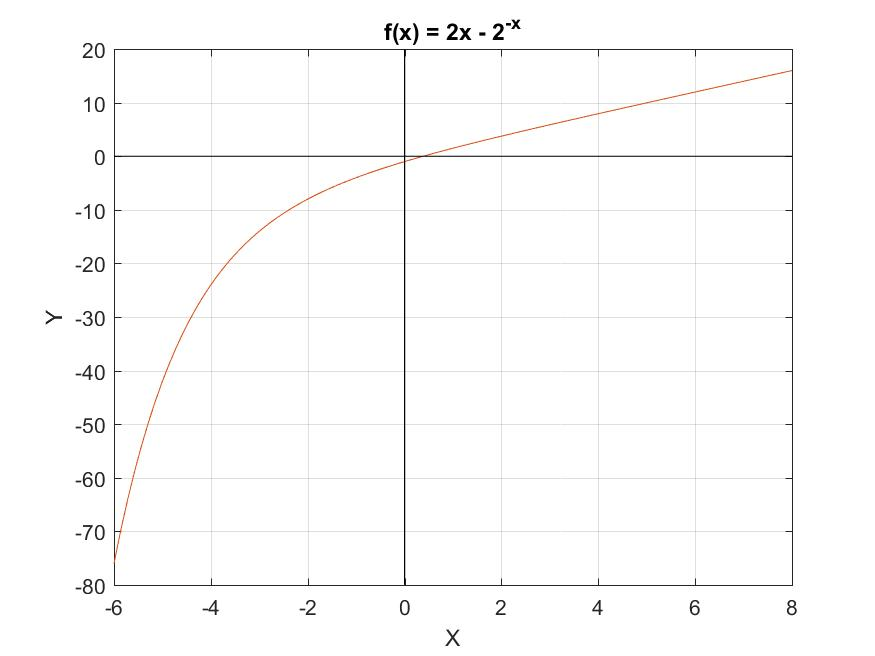
\includegraphics[width=10cm]{imagenes/NL/Funcion1.jpg}}
    Para este caso se elije el intervalo [-2 , 4].Ya que $f_{1}(x)$ decrece con mayor tasa a medida que $\bigtriangleup x$ cuando $x < 0$, tomar valores menores a $x < -2$ mal condicionarían especialmente a métodos como Regula Falsi. Los efectos de esto se pueden notar en los resultados obtenidos. Para la siguiente función se elije el intervalo [0, 3], ya que se deben cumplir requisitos de convergencia para la función utilizada en Punto Fijo. 

     \figura{Gráfico de la función no lineal 2}
    {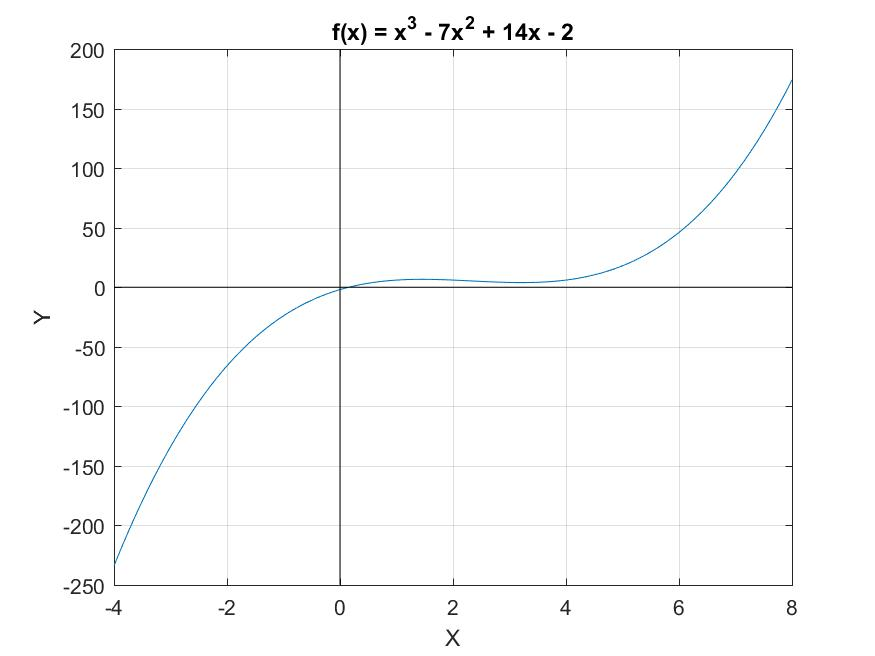
\includegraphics[width=10cm]{imagenes/NL/Funcion2.jpg}}
     
\subseccion{Tolerancia}

    Todos los métodos poseen una tolerancia de error de $10^{-15}$, por lo que para poder medir el nivel de eficacia se propone fijar el número de iteraciones como una unidad comparativa. Bajo esta base, mientras menos iteraciones requiera para llegar a una determinada precisión, más eficaz será el algoritmo en general. Existen casos donde la precisión no crece linealmente, para confirmarlo se realiza el análisis en la sección de resultados.

\subseccion{Eficiencia}

    Para efectos de pruebas, la eficiencia es medida a través del número de operaciones necesarias para entregar una solución con errores que se encuentran bajo el límite de la tolerancia propuesta. Para este caso se omiten las operaciones dependientes del software (y hardware) que implementa el método, como las asignaciones de variables o el manejo de ciclos, dejando sólo las operaciones matemáticas unitarias. Para el caso de evaluación de funciones, se fija un valor arbitrario de 5 operaciones para todas las funciones del experimento.
    

\subseccion{Optimizaciones}

Para algunos métodos es posible aplicar reglas de convergencia y métodos de optimización para acelerar la convergencia.

\begin{itemize}
    \item Los métodos de Regula Falsi, Punto Fijo y Newton determinan el punto inicial con la regla de Fourier. 
    \item Punto fijo utiliza aceleración de convergencia con Aitken y Steffensen. Se registran los resultados con y sin optimización por separado.
\end{itemize}

\subseccion{Ponderación Eficiencia versus Eficacia}
    El objetivo de este informe es determinar cual método resuelve una función en particular de mejor manera. Los criterios para determinar esto se basan en una ponderación de la eficiencia y eficacia del método. Se ha construido una heurística para calcular una magnitud por cáda método para las funciones no lineales (1) y (2). La ponderación será un valor entre 0 y 1 de manera que:
    
    Se realizarán 3 experimentos:
    \begin{enumerate} 
        \item $pondEficiencia = 0.30$ y $pondEficacia = 0.70$
        \item $pondEficiencia = 0.50$ y $pondEficacia = 0.50$
        \item $pondEficiencia = 0.70$ y $pondEficacia = 0.30$
    \end{enumerate}

\capitulo{Resultados de Métodos No Lineales}

En esta sección se presentan los gráficos resultantes de la implementación de los métodos en Matlab.

\seccion{Aproximación de la raíz}

\subseccion{Aproximación}
    Se puede observar la convergencia de la aproximación de la raíz en cada iteración.
    \figura{Aproximación de la raíz (1)} {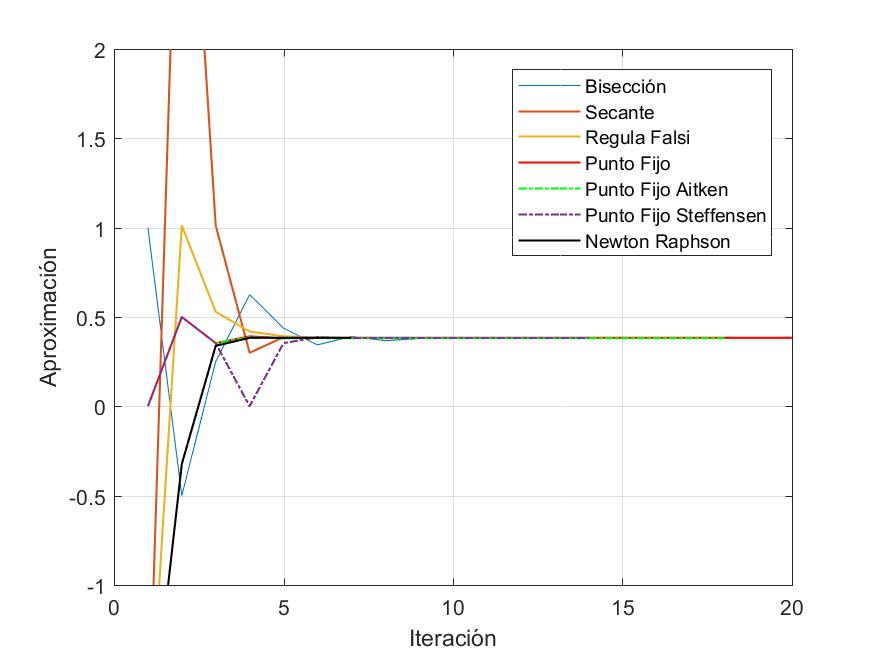
\includegraphics[width=15cm]{imagenes/NL/Aproximaciones1.jpg}}
    
\subseccion{Aproximación función 2}
    \figura{Aproximación de la raíz (2)} {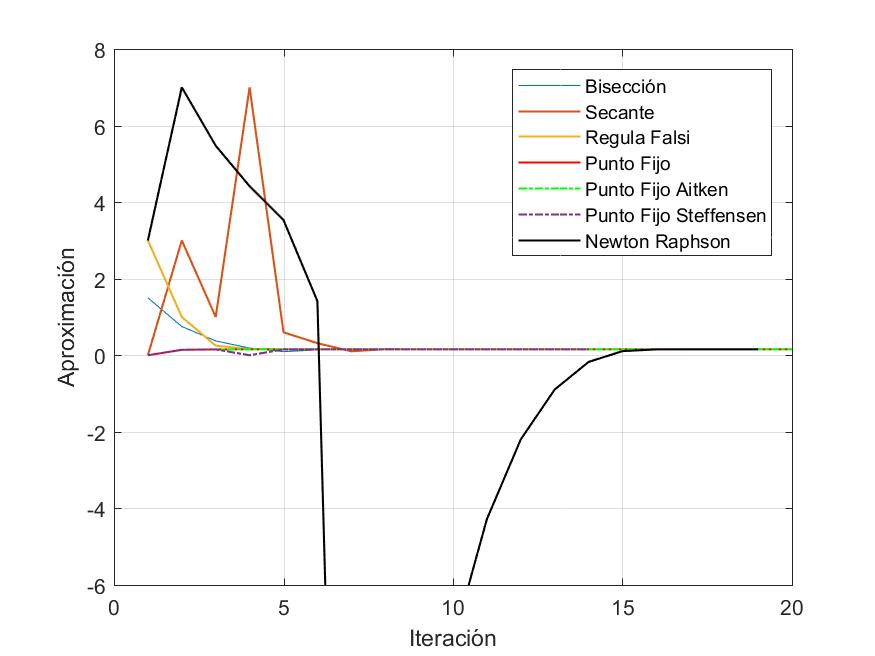
\includegraphics[width=15cm]{imagenes/NL/Aproximaciones2.jpg}}
\subseccion{Gráfico de error}
En este gráfico se puede extraer la rapidez con la que el método se acerca a la raíz. El eje Y indica el exponente de la notación $10^{-n}$. Para medir el error, se utiliza la fórmula del error relativo $e_{r}(n) = \dfrac{|x_{n}-x_{n-1}|}{|x_{n}|}$

\figura{Error (1)}
{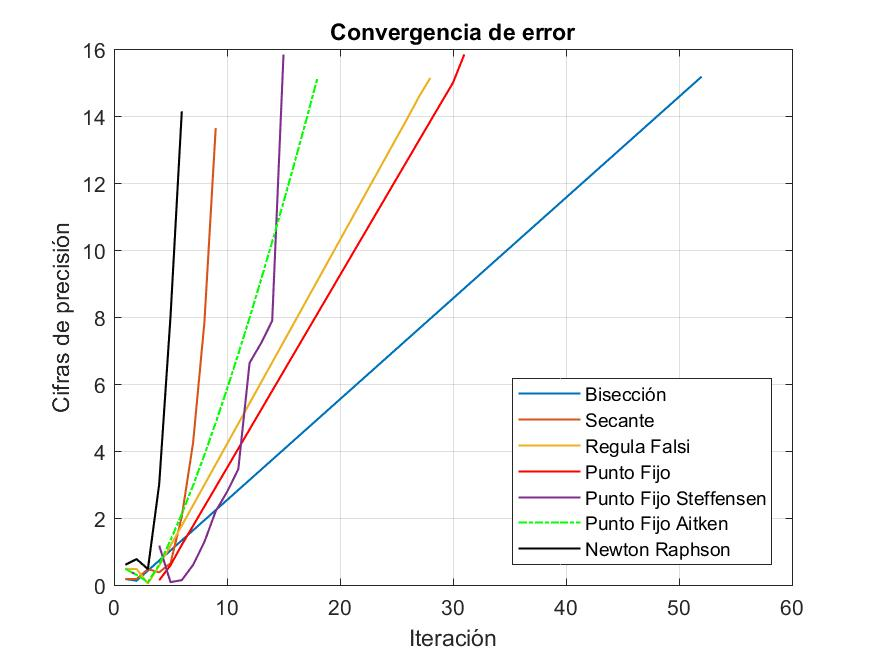
\includegraphics[width=15cm]{imagenes/NL/Errores1.jpg}}

\figura{Error (2)}
{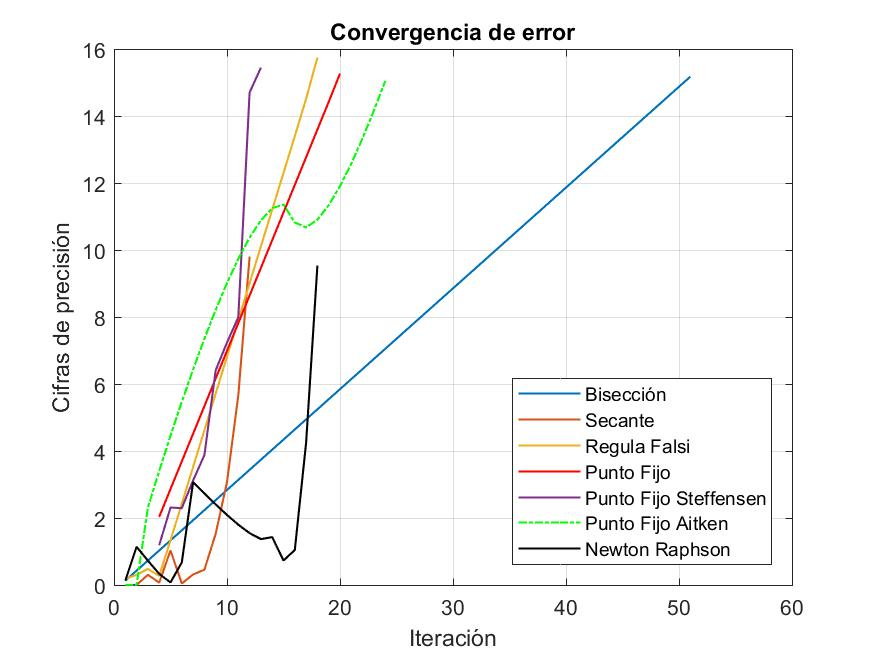
\includegraphics[width=15cm]{imagenes/NL/Errores2.jpg}}

\subseccion{Síntesis numérica}

La siguiente tabla muestra el valor de la raíz obtenido por cada método para las funciones (1) y (2)

\begin{table}[H]
\begin{tabular}{|c|c|c|c|}
\hline
\textbf{Método} & \textbf{Aproximación} & \textbf{Error} & \textbf{Iteraciones}\\ \hline
Bisección       & 0.383332347981062     & 6.661338147750939e-16  & 52\\ \hline
Punto Fijo        & 0.383332347981062     & 1.448120711012897e-16  & 29\\ \hline
Punto Fijo (Aitken) & 0.381442234672344 & 1.455296403633477e-16 & 17\\ \hline
Punto Fijo (Steffensen) & 0.383332347981062 & 8.688724266077383e-16 & 13\\ \hline
Secante         & 0.383332347981062     & 0  & 10\\ \hline
Regula Falsi    & 0.383332347981062     & 7.240603555064485e-16 & 28\\ \hline
Newton-Raphson    & 0.383332347981062     & 0 & 7\\ \hline
\end{tabular}
\caption{Resultados (1)}
\label{tab:my_label}
\end{table}

\begin{table}[H]
\centering
\begin{tabular}{|c|c|c|c|c|}
\hline
\textbf{Método} & \textbf{Aproximación} & \textbf{Error} & \textbf{Iteraciones}\\ \hline
Bisección       & 0.154533908564067     & 6.661338147750939e-16 & 52\\ \hline
Punto Fijo        & 0.154533908564067     & 5.388249583577040e-16 & 30\\ \hline
Punto Fijo (Aitken) & 0.153672207907213 & 9.030772705624057e-16 & 24\\ \hline
Punto Fijo (Steffensen) & 0.154533908564067 & 3.592166389051360e-16 & 15\\ \hline
Secante         & 0.154533908564067     & 0 & 13\\ \hline
Regula Falsi    & 0.154533908564067     & 1.796083194525679e-16 & 18\\ \hline
Newton-Raphson    & 0.154533908564067     & 0 & 19\\ \hline
\end{tabular}
\caption{Resultados (2)}
    \label{tab:my_label}
\end{table}

También se compara el error a "priori" y "posteriori" de los métodos con los valores experimentales:

\begin{table}[H]
\begin{tabular}{|c|c|c|c|}
\hline
\textbf{Método} & \textbf{Error teórico} & \textbf{Error experimental}\\ \hline
Bisección      & 6.661338147750939e-16  & 6.661338147750939e-16\\ \hline
Punto Fijo      & 1.448120711012897e-16  & 4.385786499255348e-17\\ \hline
Punto Fijo (Aitken) & 1.455296403633477e-16 & 0.001890373344365\\ \hline
Punto Fijo (Steffensen)& 8.688724266077383e-16 & 2.631471899553209e-16\\ \hline
Secante       & 0  & 0\\ \hline
Regula Falsi   & 7.240603555064485e-16 & 8.771572998510696e-17\\ \hline
Newton-Raphson  & 0 & 0\\ \hline
\end{tabular}
\caption{Comparación error teórico (1)}
\label{tab:my_label}
\end{table}

\begin{table}
\centering
\begin{tabular}{|c|c|c|}
\hline
\textbf{Método} & \textbf{Error teórico} & \textbf{Error experimental}\\ \hline
Bisección       & 6.661338147750939e-16 & 6.661338147750939e-16\\ \hline
Punto Fijo      & 5.388249583577040e-16 & 0\\ \hline
Punto Fijo (Aitken) & 9.030772705624057e-16 & 8.621082936378551e-04\\ \hline
Punto Fijo (Steffensen) & 3.592166389051360e-16 & 7.458565153307636e-17\\ \hline
Secante         & 0 & 0\\ \hline
Regula Falsi    & 1.796083194525679e-16 & 3.729282562746270e-17\\ \hline
Newton-Raphson   & 0 & 0\\ \hline
\end{tabular}
\caption{Comparación error teórico (2)}
    \label{tab:my_label}
\end{table}

\begin{table}
\centering
\begin{tabular}{|c|c|c|}
\hline
\textbf{Método} & \textbf{Error teórico} & \textbf{Error experimental}\\ \hline
Bisección       & 6.661338147750939e-16 & 1.332267629550188e-15\\ \hline
Punto Fijo      & 1.448120711012897e-16 & 0\\ \hline
Punto Fijo (Aitken) & 9.030772705624057e-16 & 8.621082936378551e-04\\ \hline
Punto Fijo (Steffensen) & 3.592166389051360e-16 & 7.458565153307636e-17\\ \hline
Secante         & 0 & 0\\ \hline
Regula Falsi    & 1.796083194525679e-16 & 3.729282562746270e-17\\ \hline
Newton-Raphson   & 0 & 0\\ \hline
\end{tabular}
\caption{Comparación error teórico (2)}
    \label{tab:my_label}
\end{table}



\subseccion{Ranking de métodos}

En base a los resultados anteriores, se procede a evaluar el desempeño de cada método y ordenarlos en un $ranking$. La heurística elegida se basa en usar el mejor método para comparar a los demás:

\[
value_{i}= pondEficiencia*\dfrac{maxOP - Op_{i}}{\bigtriangleup Eficiencia} + pondEficacia*\dfrac{maxIt - It_{i}}{\bigtriangleup Eficacia}
\]

Donde $Op_{i}$ corresponden a las operaciones para obtener tal aproximación y $It_{i}$ número de iteraciones. Además se tiene
$maxOP = max(Op_{1}, ... OP_{n})$, lo cual corresponde a la eficiencia más baja y $maxIt = max(It_{1}, ... It_{n})$ la eficacia mas baja. La variable $\bigtriangleup Eficacia$  y $\bigtriangleup Eficiencia$ es la diferencia $maxOP - minOP$ y $maxIt - minIt$, respectivamente. $value_{i}$ se encuentra en un intervalo $[0,1]$, el mejor método tendrá valor 1, mientras que los demás tendran una fracción del valor, relativo a éste. 

\figura{Ranking Eficacia: 50 Eficiencia: 50 (1)}
{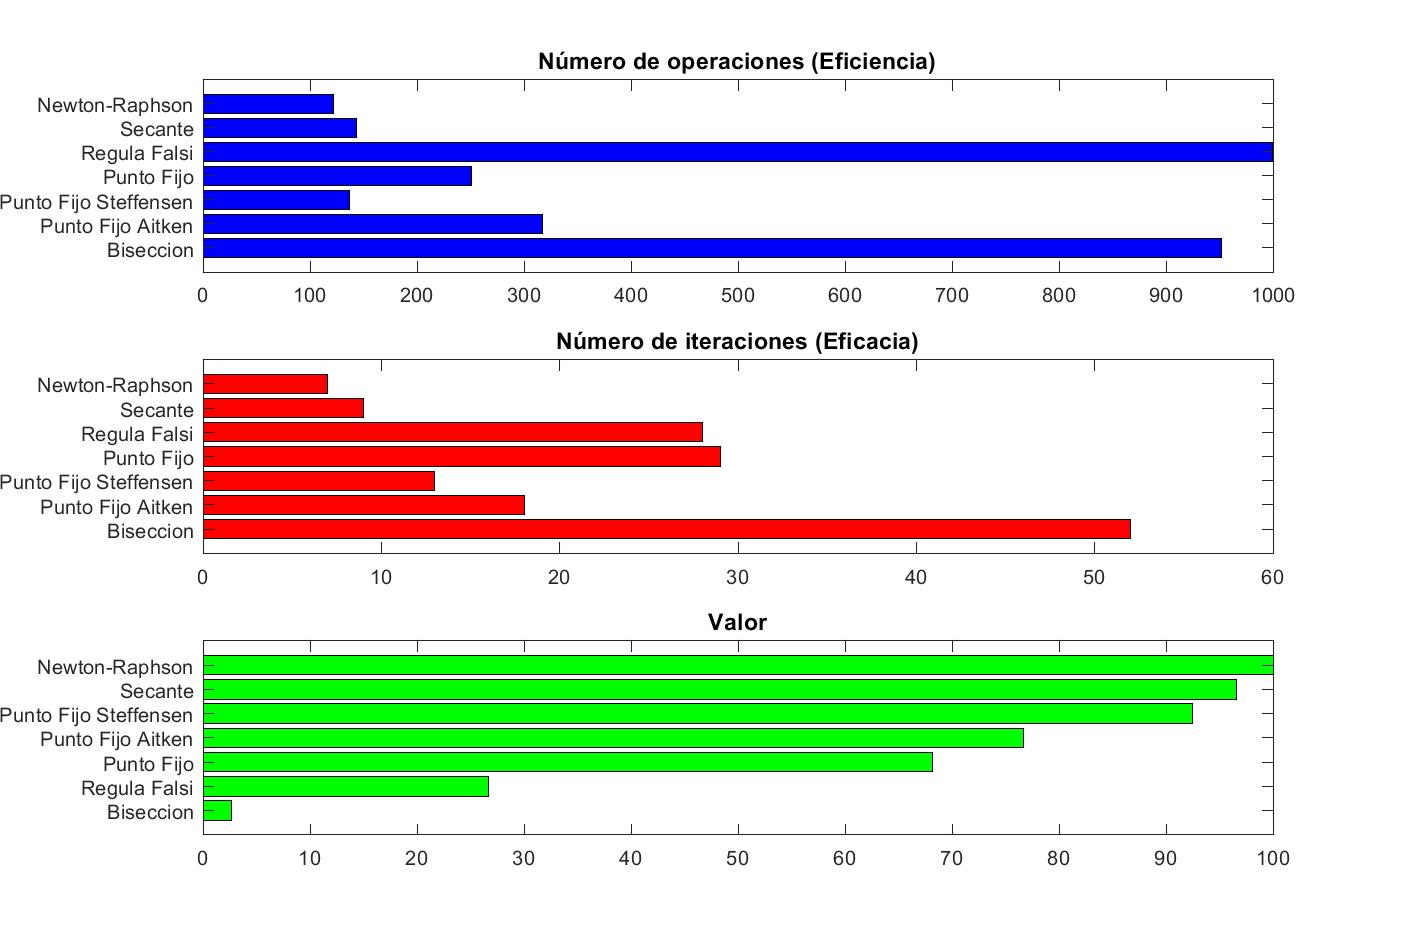
\includegraphics[width=15cm]{imagenes/NL/ranking1-1.jpg}}

\figura{Ranking Eficacia: 30 Eficiencia: 70 (1)}
{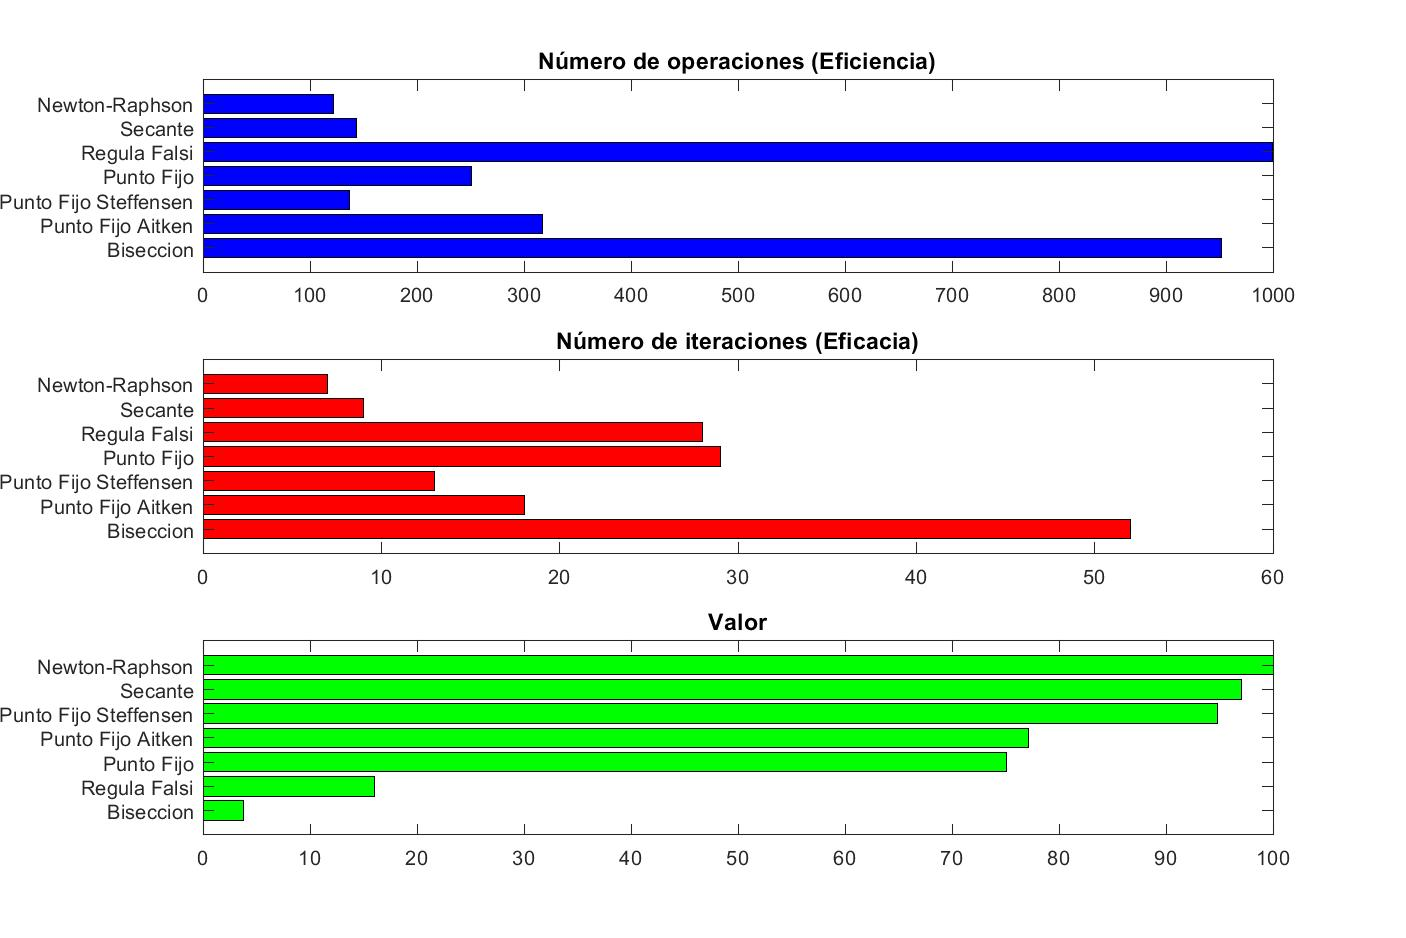
\includegraphics[width=15cm]{imagenes/NL/ranking1-2.jpg}}

\figura{Ranking Eficacia: 70 Eficiencia: 30 (1)}
{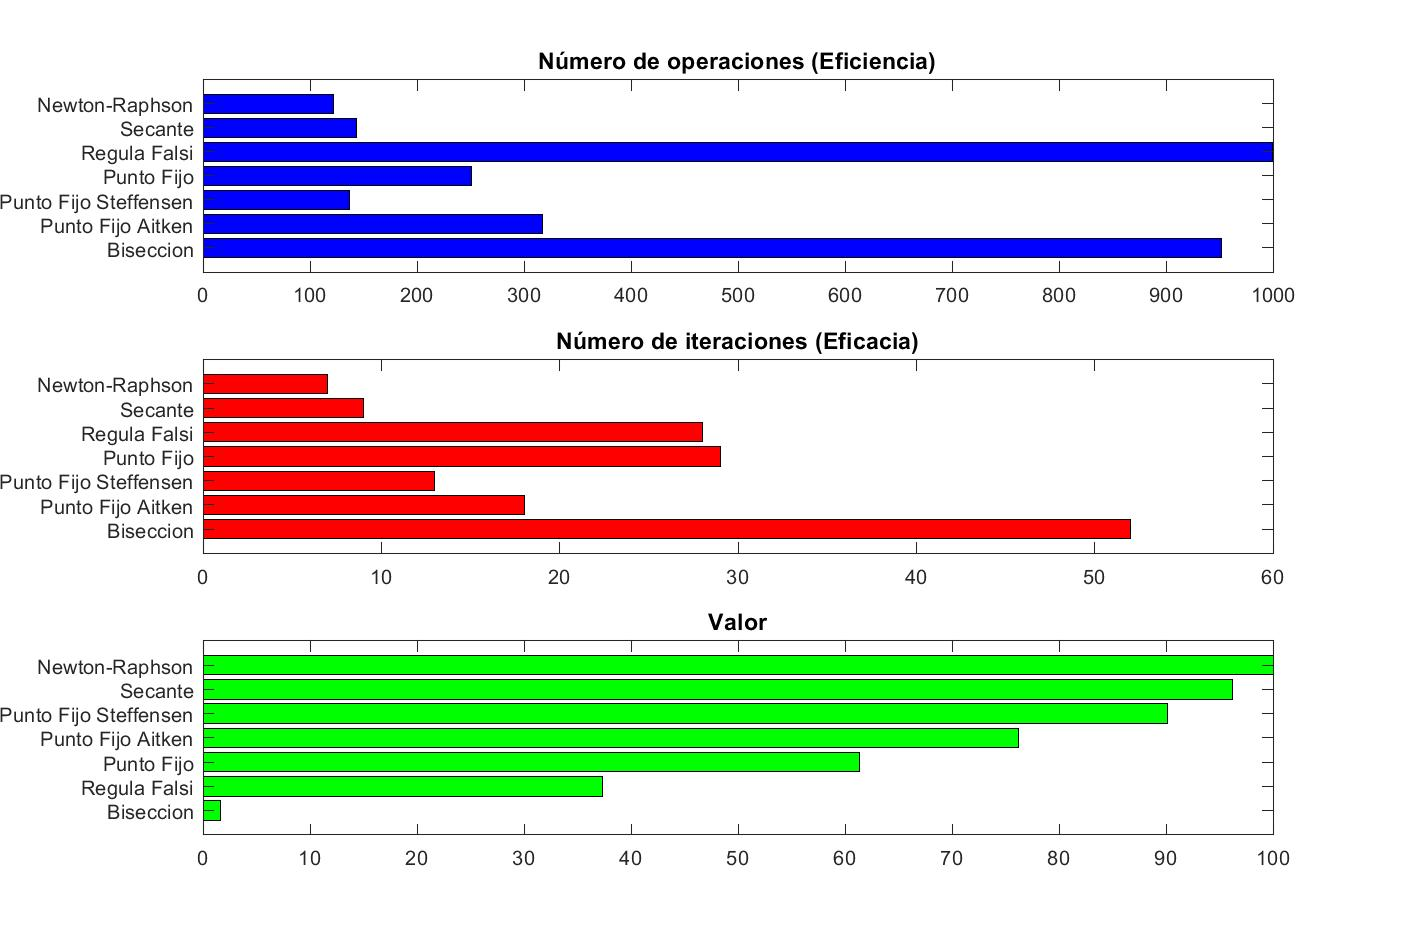
\includegraphics[width=15cm]{imagenes/NL/ranking1-3.jpg}}

\figura{Ranking Eficacia: 50 Eficiencia: 50 (2)}
{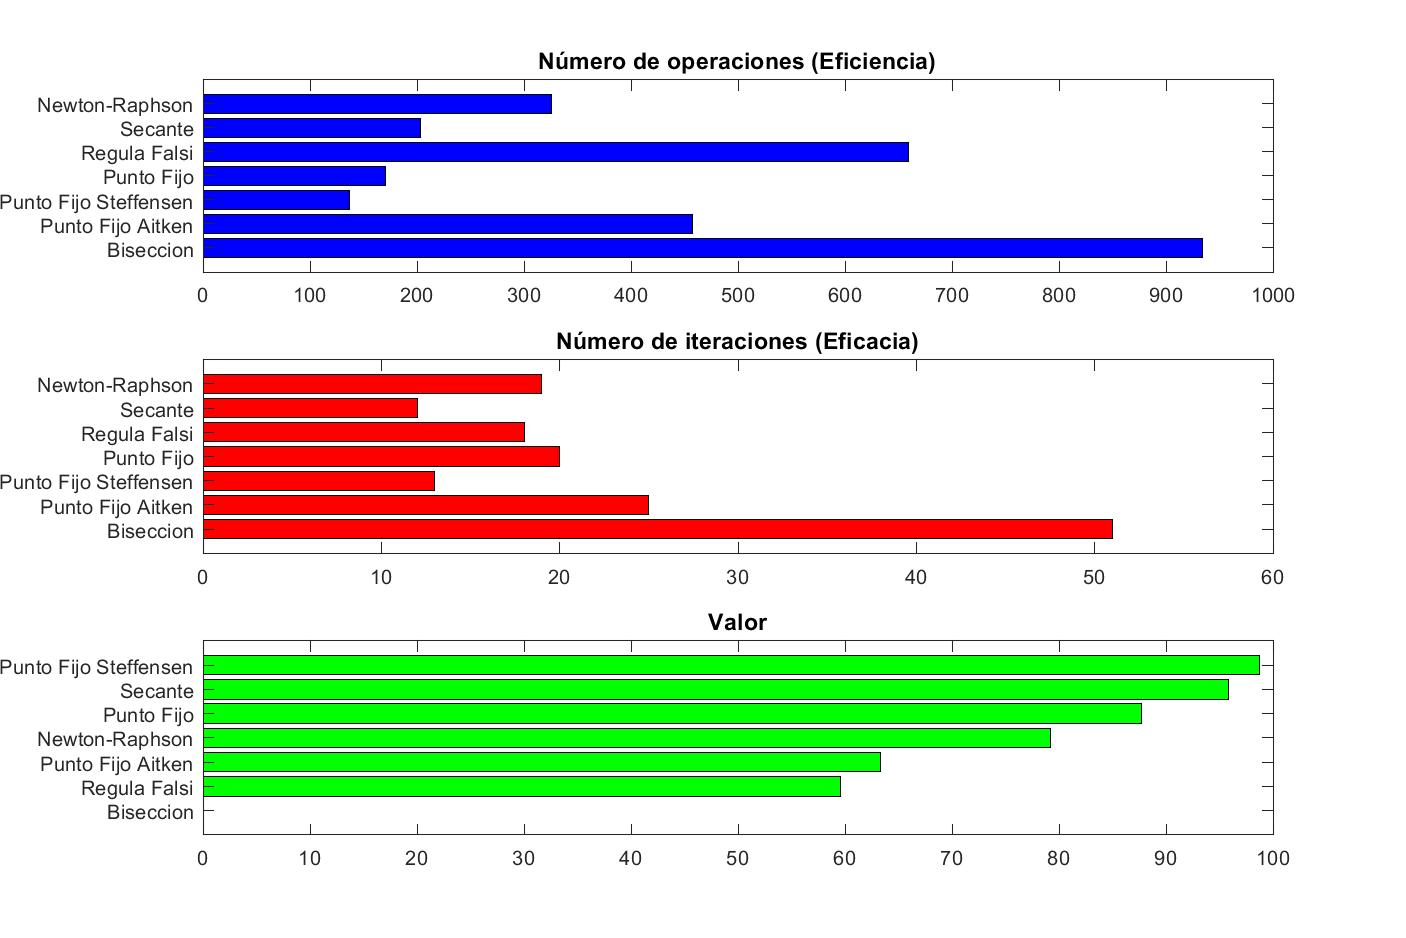
\includegraphics[width=15cm]{imagenes/NL/ranking2-1.jpg}}

\figura{Ranking Eficacia: 30 Eficiencia: 70 (2)}
{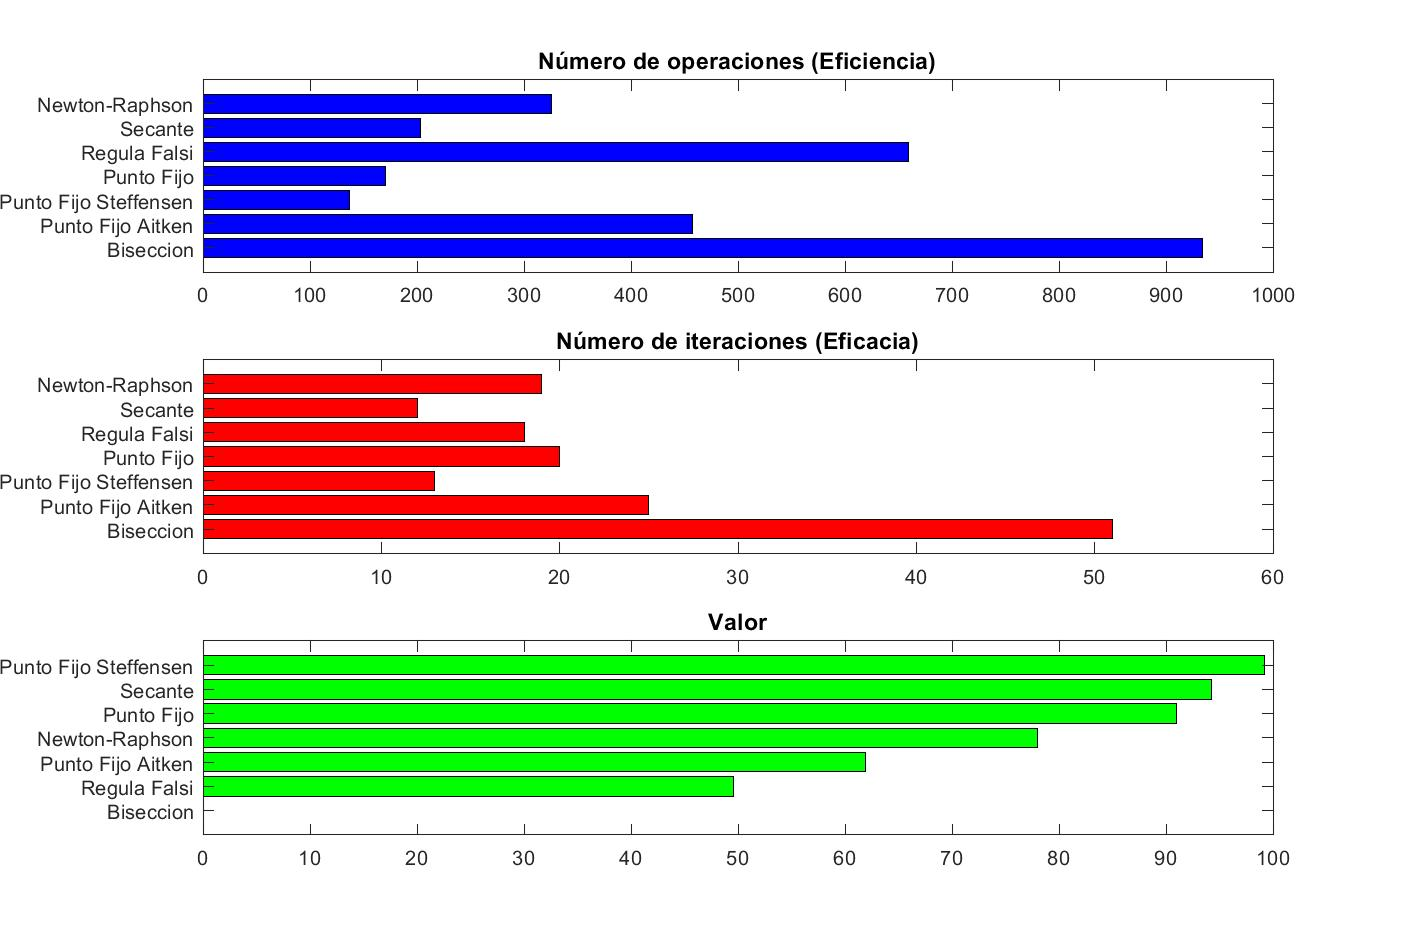
\includegraphics[width=15cm]{imagenes/NL/ranking2-2.jpg}}

\figura{Ranking Eficacia: 70 Eficiencia: 30 (2)}
{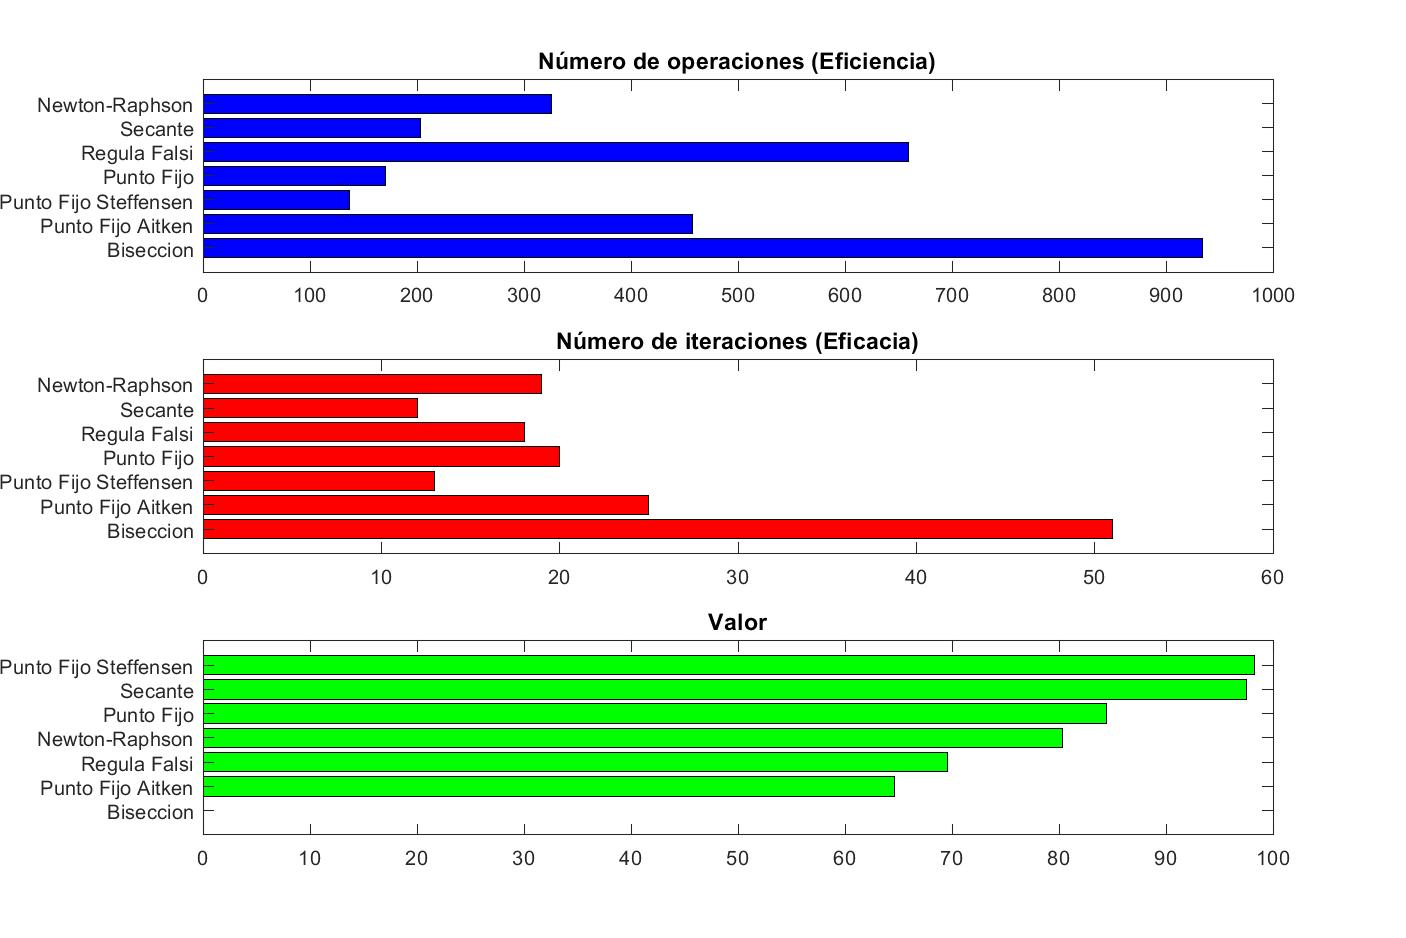
\includegraphics[width=15cm]{imagenes/NL/ranking2-3.jpg}}

\subseccion{Resultados Newton Multivariable}

Para el primer sistema de ecuaciones (3) se tiene el siguiente gráfico de error
    
\figura{Error Newton Multivariable (3)}
{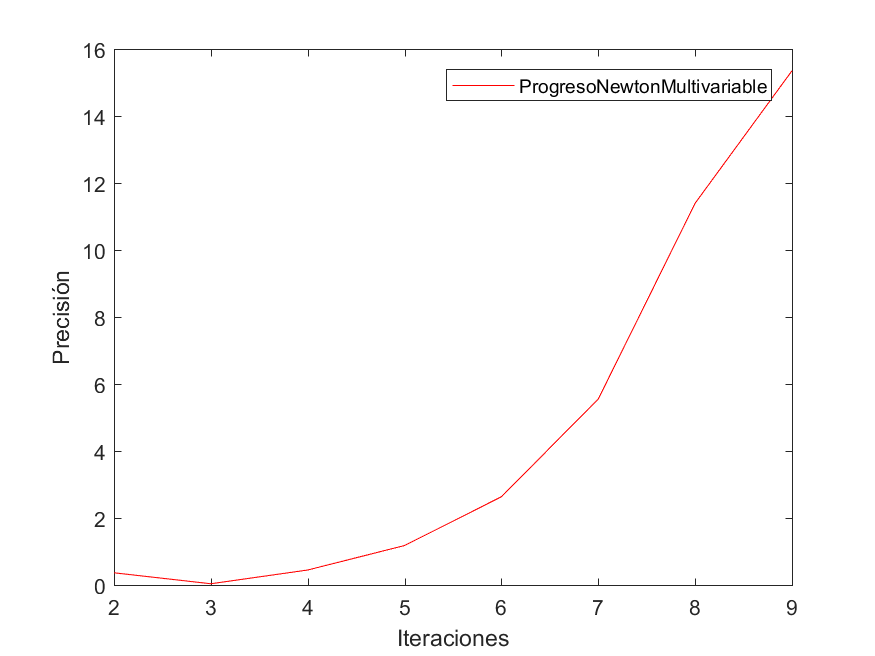
\includegraphics[width=15cm]{imagenes/NL/NewtonMultivariable_performance.png}}

\begin{table}[]
\centering
\begin{tabular}{|c|c|c|c|c|}
\hline
\textbf{$x_{1}$} & \textbf{$x_{2}$} & \textbf{Error} & \textbf{Iteraciones} & \textbf{Operaciones}\\ \hline
2.193439415415308 & 3.020466468123034  & 4.440892098500626e-16     & 9 & 546\\ \hline
\end{tabular}
\caption{Síntesis Newton Multivariable (3)}
    \label{tab:my_label}
\end{table}

\capitulo{Análisis de resultados}


\seccion{Métodos no lineales}

Para ambas funciones se opta por utilizar un gráfico de error donde se visualice claramente la rapidez de convergencia del error. Otra manera de graficar esto es observar como todas convergen a 0, sin embargo de esta forma las funciones tenderían a entrecruzarse y dificultar la visibilidad.

Respecto a la comparación con el error teórico, Secante y Newton-Raphson
se anulan y no logran dar un error (a diferencia de que el error sea tan pequeño que se aproxime a 0). Los otros errores teóricos entregan un valor más pequeño que el experimental, posiblemente porque los cálculos son más sensibles en esas magnitudes. Para el caso de Aitken, al haber una convergencia a otro valor, el error experimental se mide relativo a otro valor, por tanto el valor teórico coincide con la distancia a la raíz. 

\subseccion{Análisis Función 1}

Comenzando con la función $f_{1}(x)=2x - 2^{-x}$, se puede notar que todas los métodos convergen al mismo número, siendo Newton-Raphson y Secante los que obtienen la máxima precisión - la precisión es tal que no puede ser almacenado por un sistema de 64 bits - , por lo que se aproxima $error = 0$ y produciendo un corte en la curva. Además, ambos métodos convergen de manera no lineal (se corrobora con la teoría), mientras que los demás métodos crecen linealmente o tienen oscilaciones causadas por el condicionamiento. Entre todos los métodos, Aitken presenta estas oscilaciones durante las aproximaciones, razón por la cual se puede asociar a una raíz no tan precisa como los otros métodos. En cuanto al ranking de las figuras 4-5, 4-6 y 4-7, los métodos de Newton-Raphson, Punto Fijo con Steffensen y Secante son los mejores para la función (1), tanto en eficiencia como en eficacia, sin embargo el método Secante posee la ventaja de no requerir el cálculo de la derivada ni la aplicación de la regla de Fourier, mientras que Punto Fijo (Steffensen) es la que utiliza menos operaciones entre todos los métodos. También se puede notar que Regula Falsi realiza más operaciones para llegar al resultado, a pesar de que es la tercera mejor en cuanto a iteraciones. Otro punto que se debe tener en cuenta es que Regula Falsi y Punto fijo depende mucho del condicionamiento del problema
el primero ya que la secante que forman los puntos utilizados se asemeja a la curva misma, realizando iteraciones que se aproximan lentamente hacia la raíz.

\subseccion{Análisis Función 2}

Para la gráfica de convergencia de la figura 3-2, se muestra que todas convergen al resultado, sin embargo Punto Fijo con Aitken diverge en magnitudes de $10^{-3}$. Lo primero en destacar es el rápido cambio de Newton-Raphson, lo cual se asocia a la derivada en particular en ese punto, sin embargo el error disminuye en orden cuadrático como es esperado. Se puede notar con claridad que Regula Falsi cambia su eficiencia con respecto al experimento anterior.
Se comprueba que el método Bisección se mantiene independiente de la función, pero no logra un buen desempeño en ningún caso. También cabe mencionar que los métodos no fueron afectados por la forma de esta curva, pero el resultado puede ser otro al experimentar con raíces múltiples. 
Respecto a la heurística aplicada, Newton-Raphson se mantiene como el mejor método en funciones forma polinomial.

\capitulo{Sistemas de ecuaciones lineales}

En este capítulo se implementan y analizan los siguientes métodos sobre sistemas de ecuaciones:

\begin{itemize}
    \item Iterativos:
    \begin{itemize}
        \item Gauss-Jacobi
        \item Gauss-Seidel
    \end{itemize}
    \item Directos:
    \begin{itemize}
        \item Factorización LU
        \item QR
        \item Cholesky
    \end{itemize}
\end{itemize}

Todos los métodos son aplicados para resolver el sistema $Ax = b$ , en tres experimentos, donde:
\begin{itemize}
    \item $A_{1} \in {\rm I\!R}^{(289, 289)}$, $b_{1} \in {\rm I\!R}^{(289, 1)} $ (1)
    \item $A_{2} \in {\rm I\!R}^{(1089, 1089)}$, $b_{2} \in {\rm I\!R}^{(1089, 1)} $ (2)
    \item $A_{3} \in {\rm I\!R}^{(4225, 4225)}$, $b_{3} \in {\rm I\!R}^{(4225, 1)}$ (3)
\end{itemize}

Existen condiciones para poder aplicar estos métodos para resolver estos sistemas, para efectos del experimento, las matrices proporcionadas cumplen con todas estas condiciones:

\begin{itemize}
    \item La matriz es cuadrada: Si no lo fuera, sólo el método QR podría aplicarse directamente, teniendo que pasar por un proceso de ortogonalización lo cual no corresponde a los alcances de este informe.
    \item La matriz es Hermitiana y declarada positiva: Se requiere para el método de Cholesky, de manera que se posibilite la factorización $A = LL^t$. Nuevamente, esta propiedad no está en los alcances del informe.
    \item La matriz es diagonal estrictamente dominante: De cumplirse, se puede garantizar que los métodos Gauss-Seidel y Gauss-Jacobi convergen a la solución.
\end{itemize}

Los experimentos consisten en resolver (1), (2) y (3), para luego utilizar el mismo modelo heurístico de capítulos anteriores para determinar el método más apto para resolver un determinado problema.

\subseccion{Eficacia del Método}

Ya que se va a comparar métodos iterativos y directos, no es posible aplicar el número de iteraciones como criterio en el cálculo de la eficacia. Dado que no hay un límite definido para el error aceptado, se puede considerar el error relativo final como una buena escala de comparación de la eficacia.

Para el error relativo se utiliza la norma infinita dado por la siguiente ecuación, sea vector solución real $X$ y la aproximación final $\hat{X}$:\\
\begin{center}
$err = \dfrac{||\hat{X} - X||_{\infty}}{||X||_{\infty}}$
\end{center}

Recordar que la norma infinita para una matriz $(n,m)$ usando las columnas corresponde a $max_{1 \leq i \leq n}\sum_{j=1}^{m}|a_{i,j}|$

Como referencia al valor real (para el cálculo de error) se utiliza la función $linsolve$ de Matlab.

\subseccion{Eficiencia del Método}

Al igual que con los métodos no lineales, se procede a calcular el número de operaciones como un indicador de la eficiencia para ambos métodos. Como se aplican matrices de grandes dimensiones, el número de operaciones va a diferir en grandes magnitudes entre distintos métodos, por lo que se aplica una escala logarítmica.

\seccion{Resultados Sistemas de ecuaciones}

En las siguientes figuras se grafica la matriz solución del sistema para cada método.

% INICIO 289X289

\begin{center}
\figura{Gauss-Jacobi 289X289}
{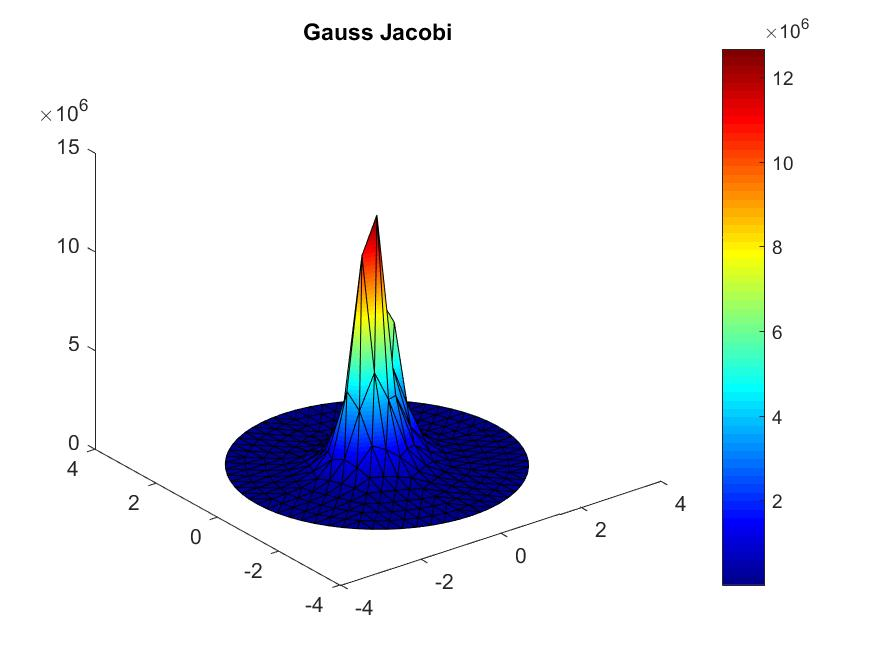
\includegraphics[width=16cm]{imagenes/SE/Resultados289_GJ.jpg}}
\end{center}

\figura{Gauss-Seidel 289X289}
{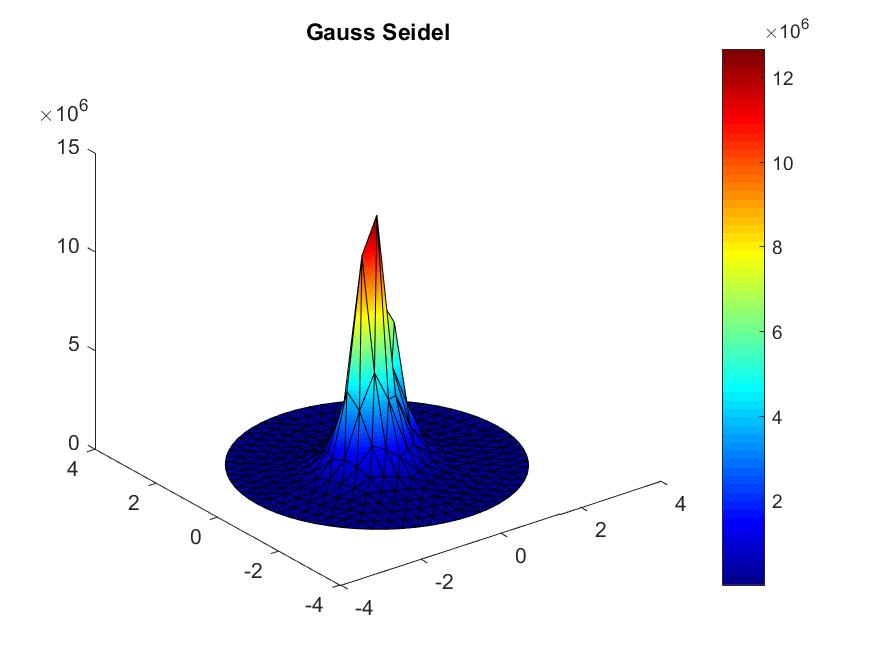
\includegraphics[width=16cm]{imagenes/SE/Resultados289_GS.jpg}}

\figura{Factorización LU 289X289}
{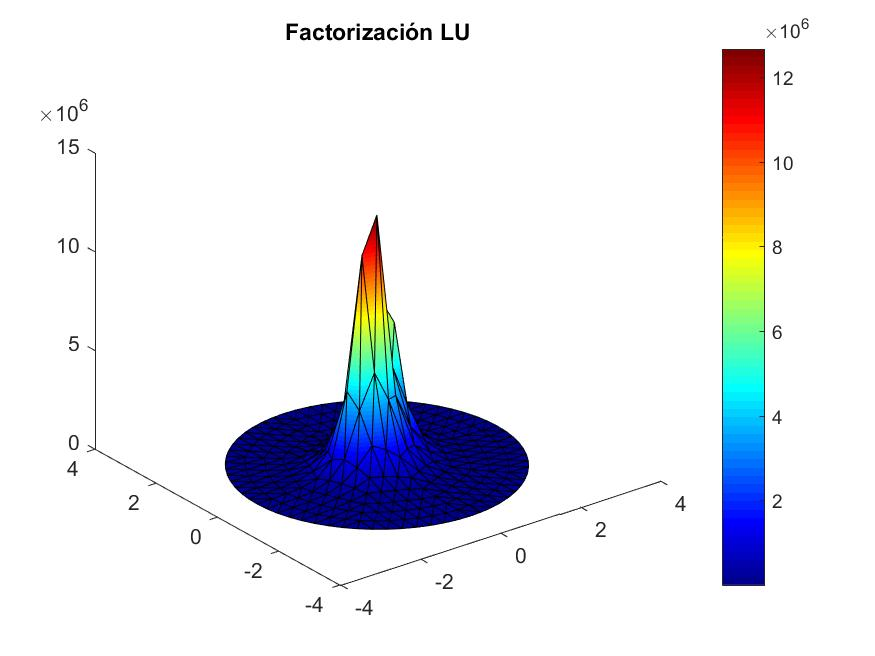
\includegraphics[width=16cm]{imagenes/SE/Resultados289_LU.jpg}}

\figura{Factorización QR 289X289}
{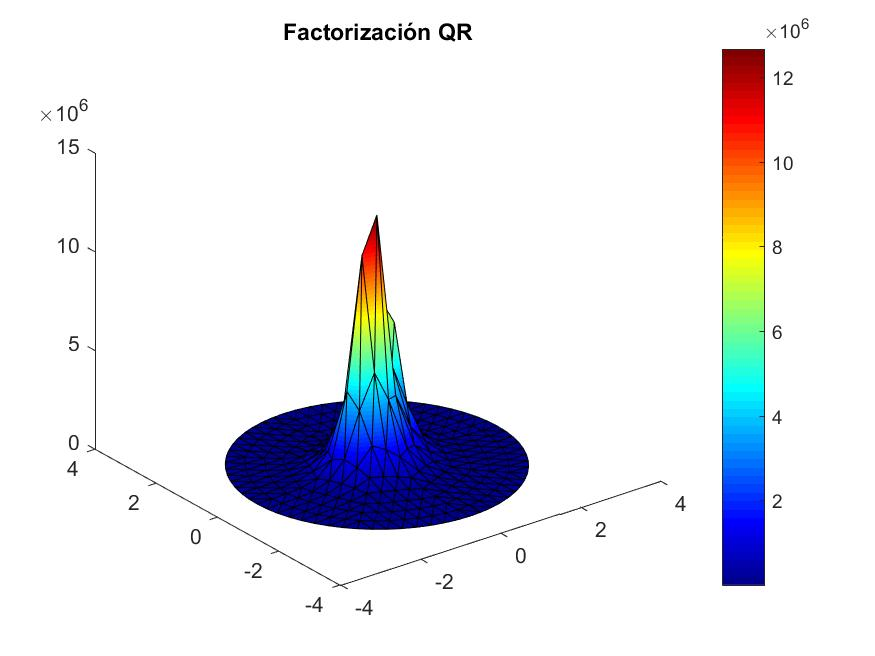
\includegraphics[width=16cm]{imagenes/SE/Resultados289_QR.jpg}}

\figura{Cholesky 289X289}
{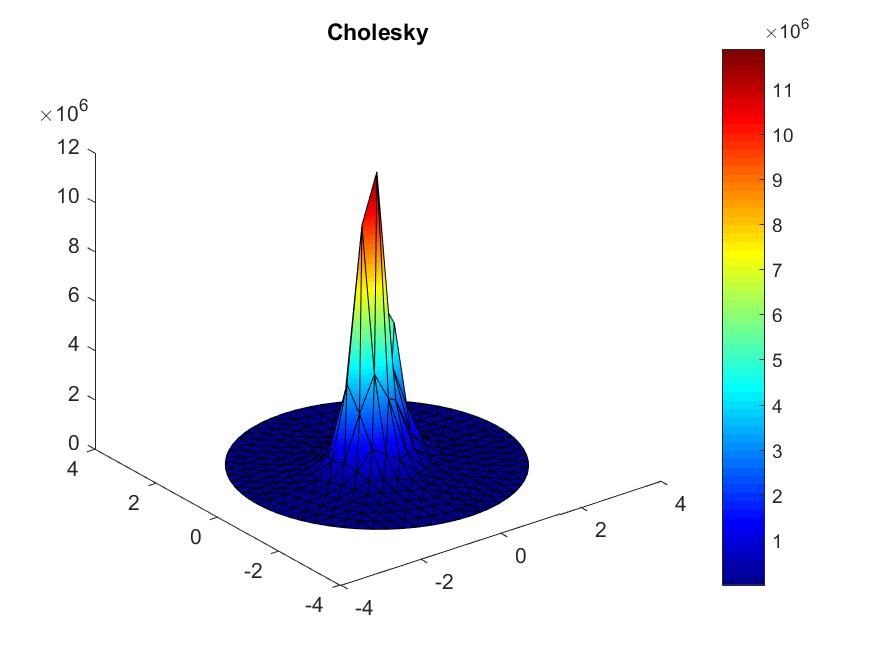
\includegraphics[width=16cm]{imagenes/SE/Resultados289_Ch.jpg}}
% FIN 289X289

Luego, para el sistema 1089x1089 se tienen los siguientes resultados.

% INICIO 1089X1089

\figura{Gauss-Jacobi 1089X1089}
{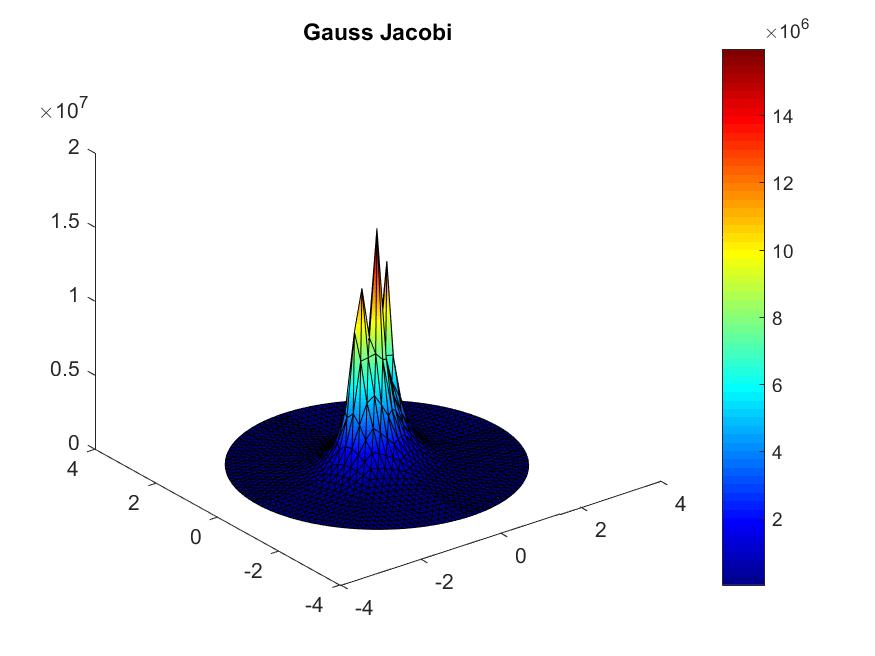
\includegraphics[width=16cm]{imagenes/SE/Resultados1089_GJ.jpg}}

\figura{Gauss-Seidel 1089X1089}
{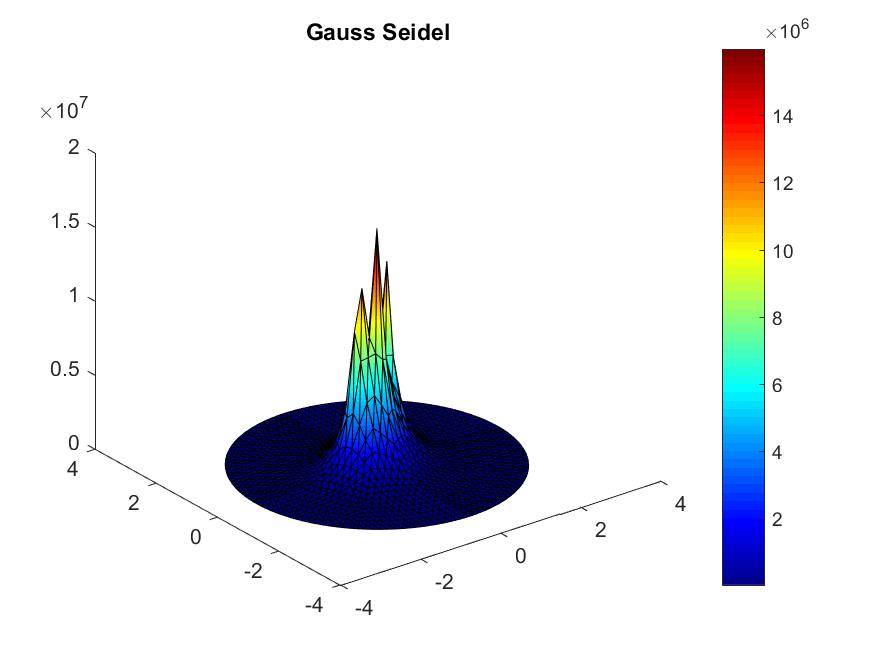
\includegraphics[width=16cm]{imagenes/SE/Resultados1089_GS.jpg}}

\figura{Factorización LU 1089X1089}
{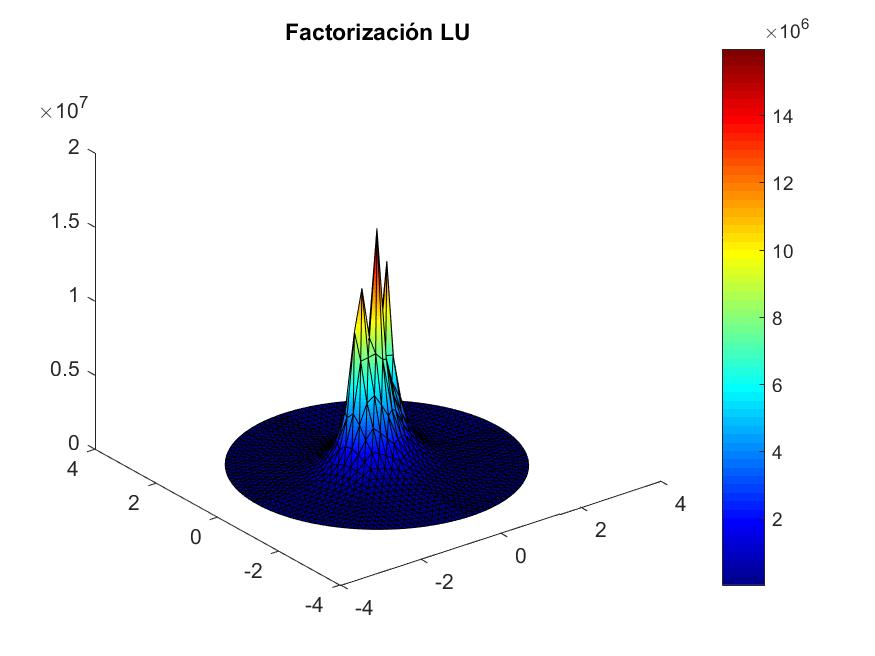
\includegraphics[width=16cm]{imagenes/SE/Resultados1089_LU.jpg}}

\figura{Factorización QR 1089X1089}
{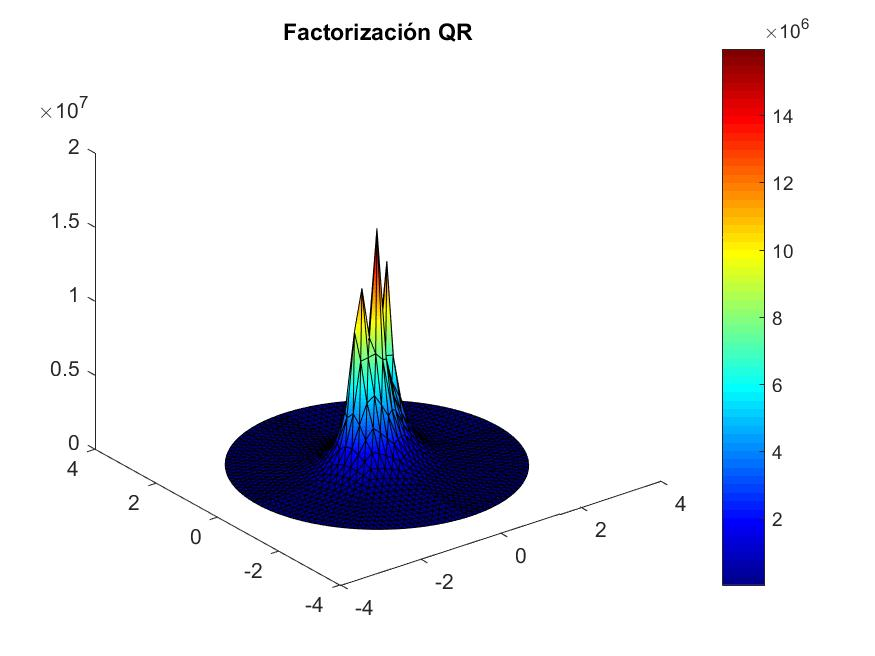
\includegraphics[width=16cm]{imagenes/SE/Resultados1089_QR.jpg}}

\figura{Cholesky 1089X1089}
{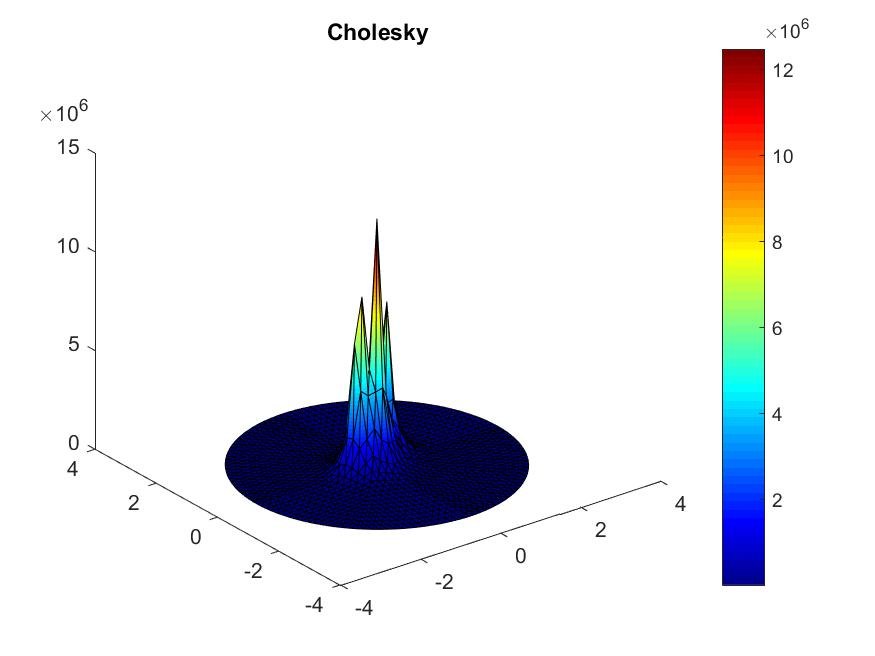
\includegraphics[width=16cm]{imagenes/SE/Resultados1089_Ch.jpg}}
% FIN 1089X1089

Y para el sistema $4225x4225$:
% INICIO 4225X4225

\figura{Gauss-Jacobi 4225X4225}
{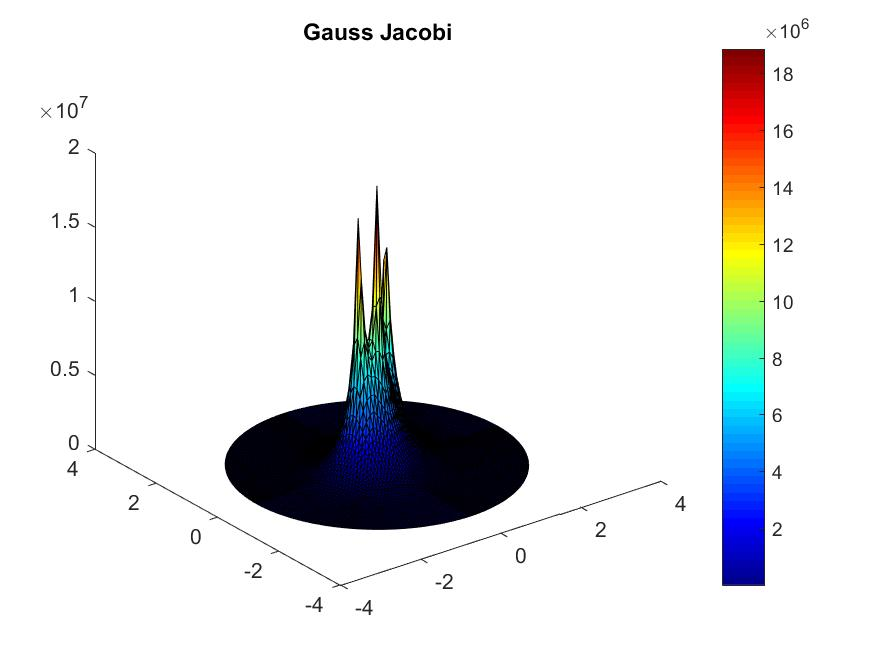
\includegraphics[width=16cm]{imagenes/SE/Resultados4225_GJ.jpg}}

\figura{Gauss-Seidel 4225X4225}
{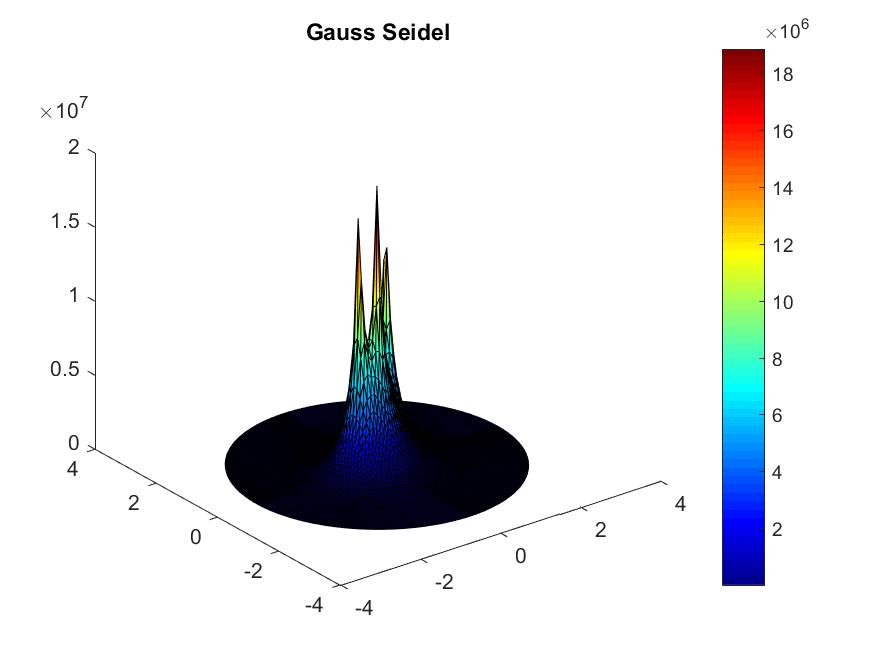
\includegraphics[width=16cm]{imagenes/SE/Resultados4225_GS.jpg}}

\figura{Factorización LU 4225X4225}
{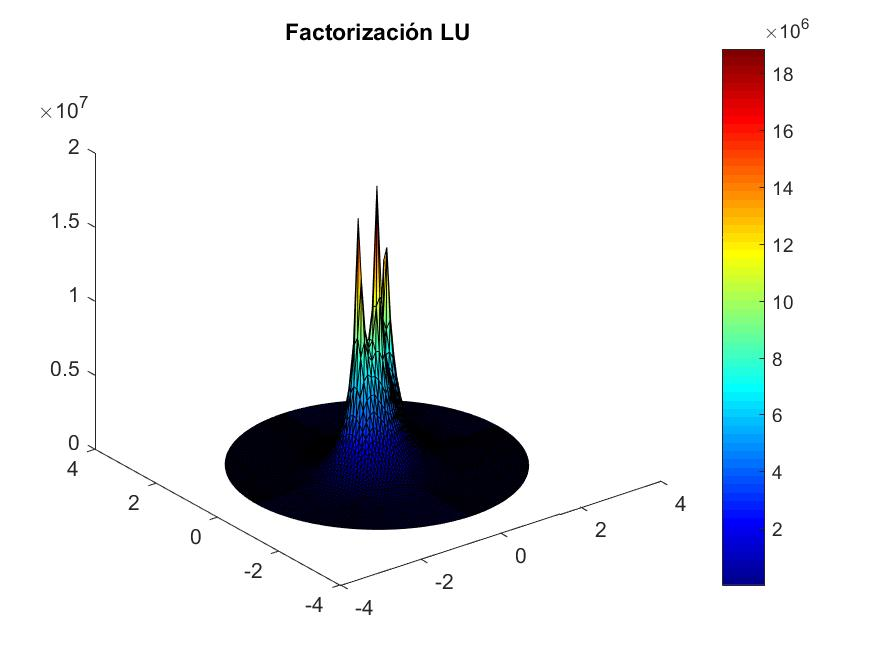
\includegraphics[width=16cm]{imagenes/SE/Resultados4225_LU.jpg}}

\figura{Factorización QR 4225X4225}
{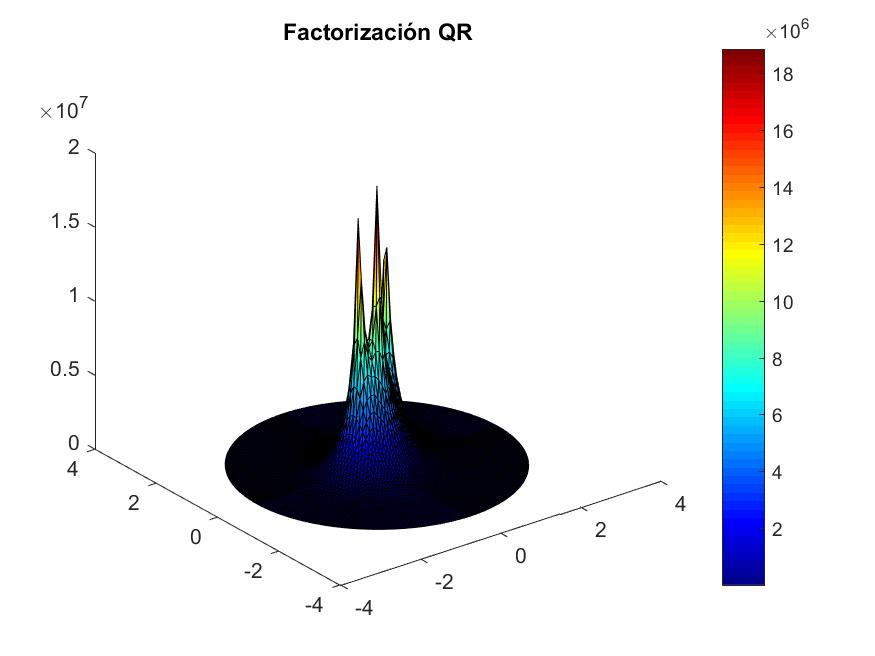
\includegraphics[width=16cm]{imagenes/SE/Resultados4225_QR.jpg}}

\figura{Cholesky 4225X4225}
{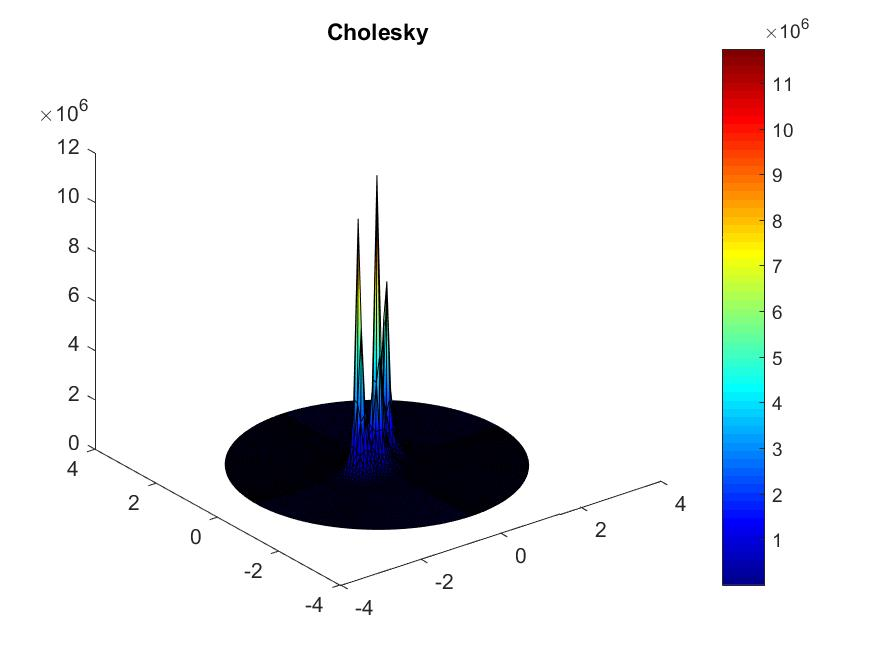
\includegraphics[width=16cm]{imagenes/SE/Resultados4225_Ch.jpg}}
% FIN 4225X4225

Se obtiene el siguiente gráfico que visualiza la valoración para cada método. Para visualizar estos gráficos se debe tener en cuenta que las ponderaciones se denotan por el orden Eficiencia - Eficacia.

\figura{Resultados Sistema 289x289}
{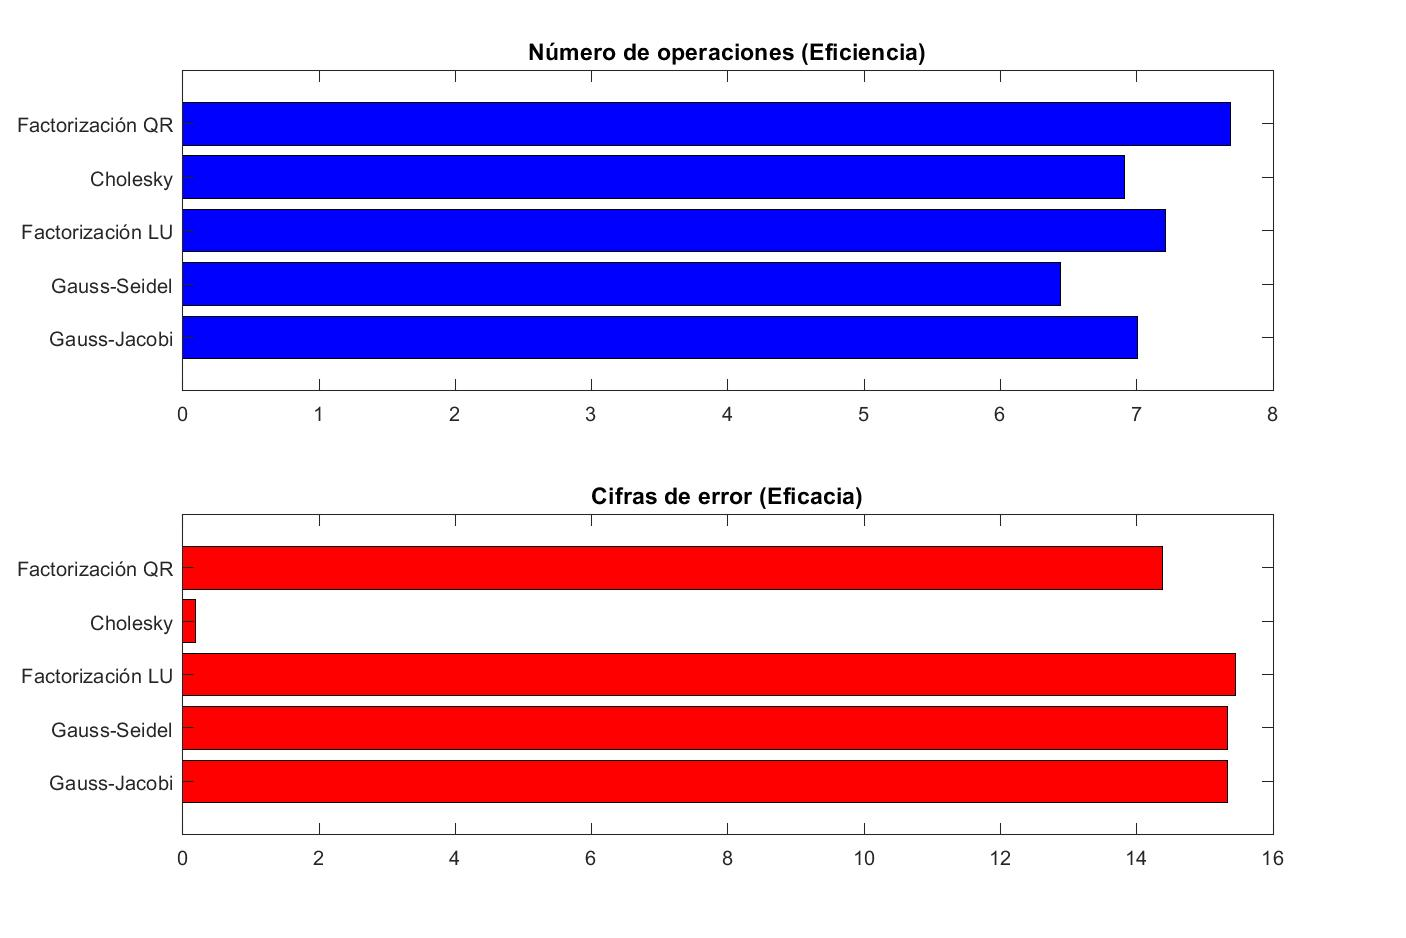
\includegraphics[width=15cm]{imagenes/SE/SE289.jpg}}

\figura{Ranking Sistema 289x289}
{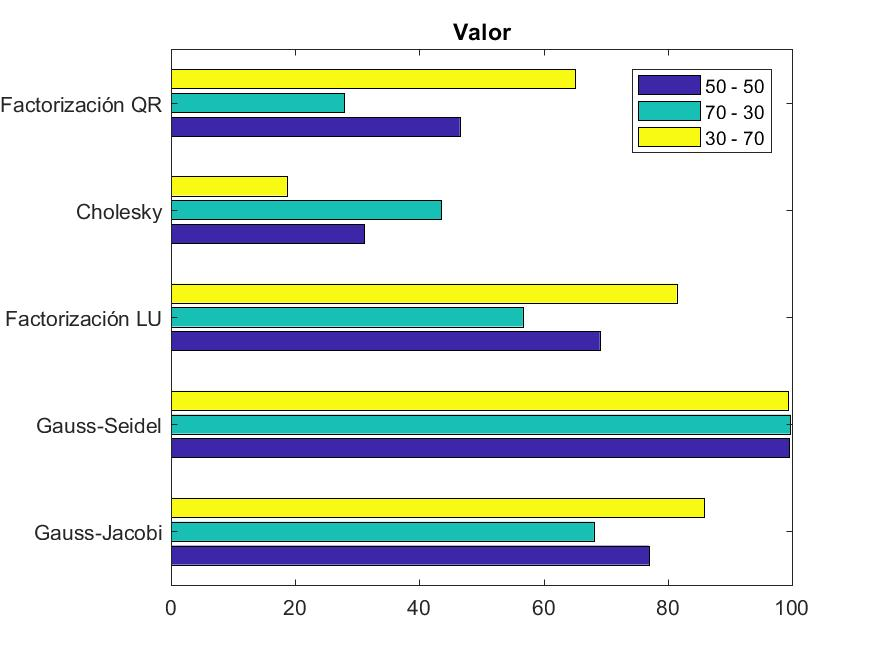
\includegraphics[width=15cm]{imagenes/SE/ranking289.jpg}}

\figura{Resultados Sistema 1089x1089}
{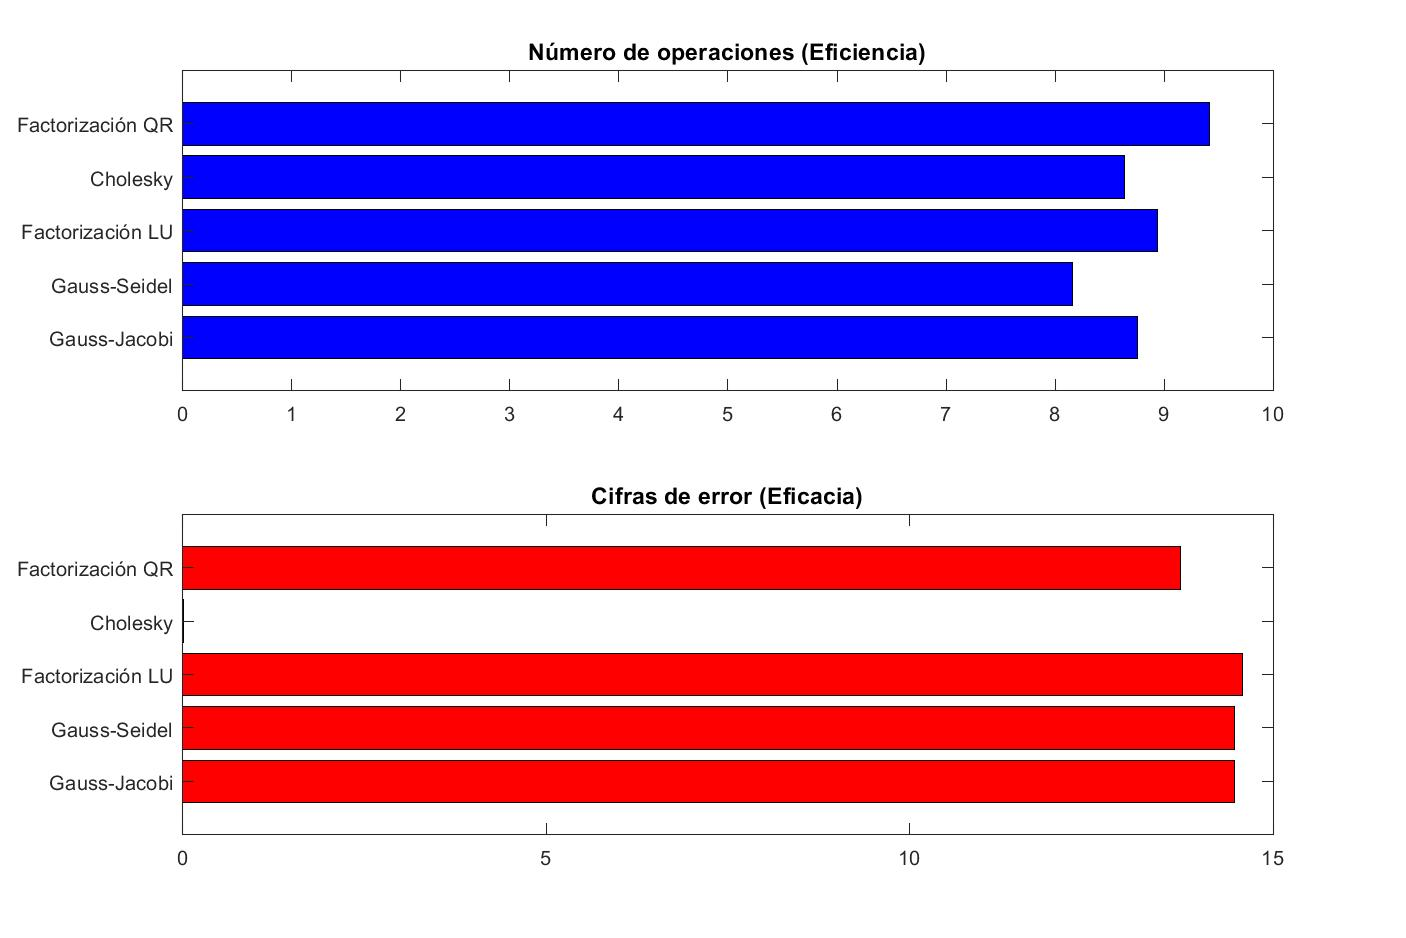
\includegraphics[width=15cm]{imagenes/SE/SE1089.jpg}}

\figura{Ranking Sistema 1089x1089}
{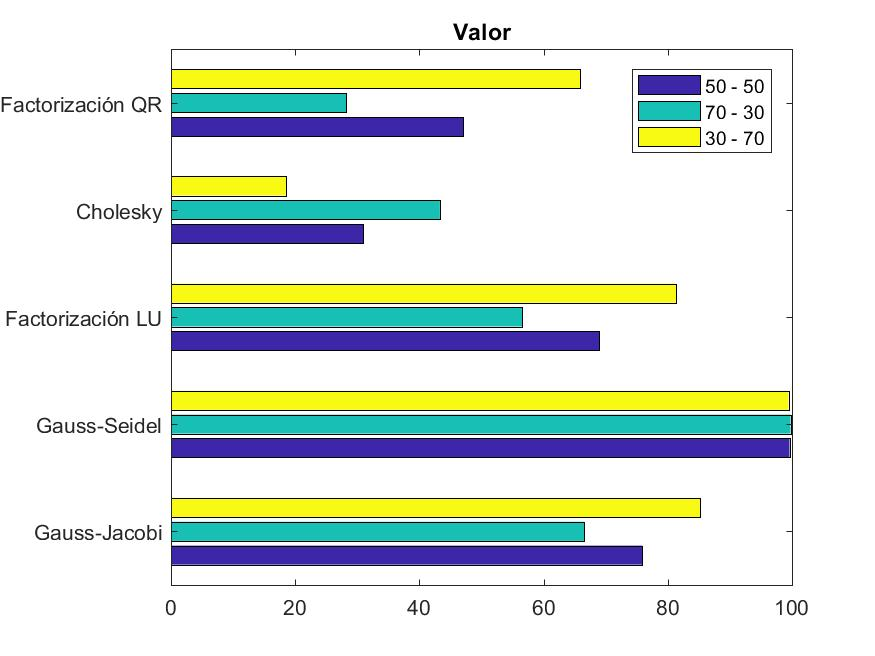
\includegraphics[width=15cm]{imagenes/SE/ranking1089.jpg}}

\figura{Resultados Sistema 4225x4225}
{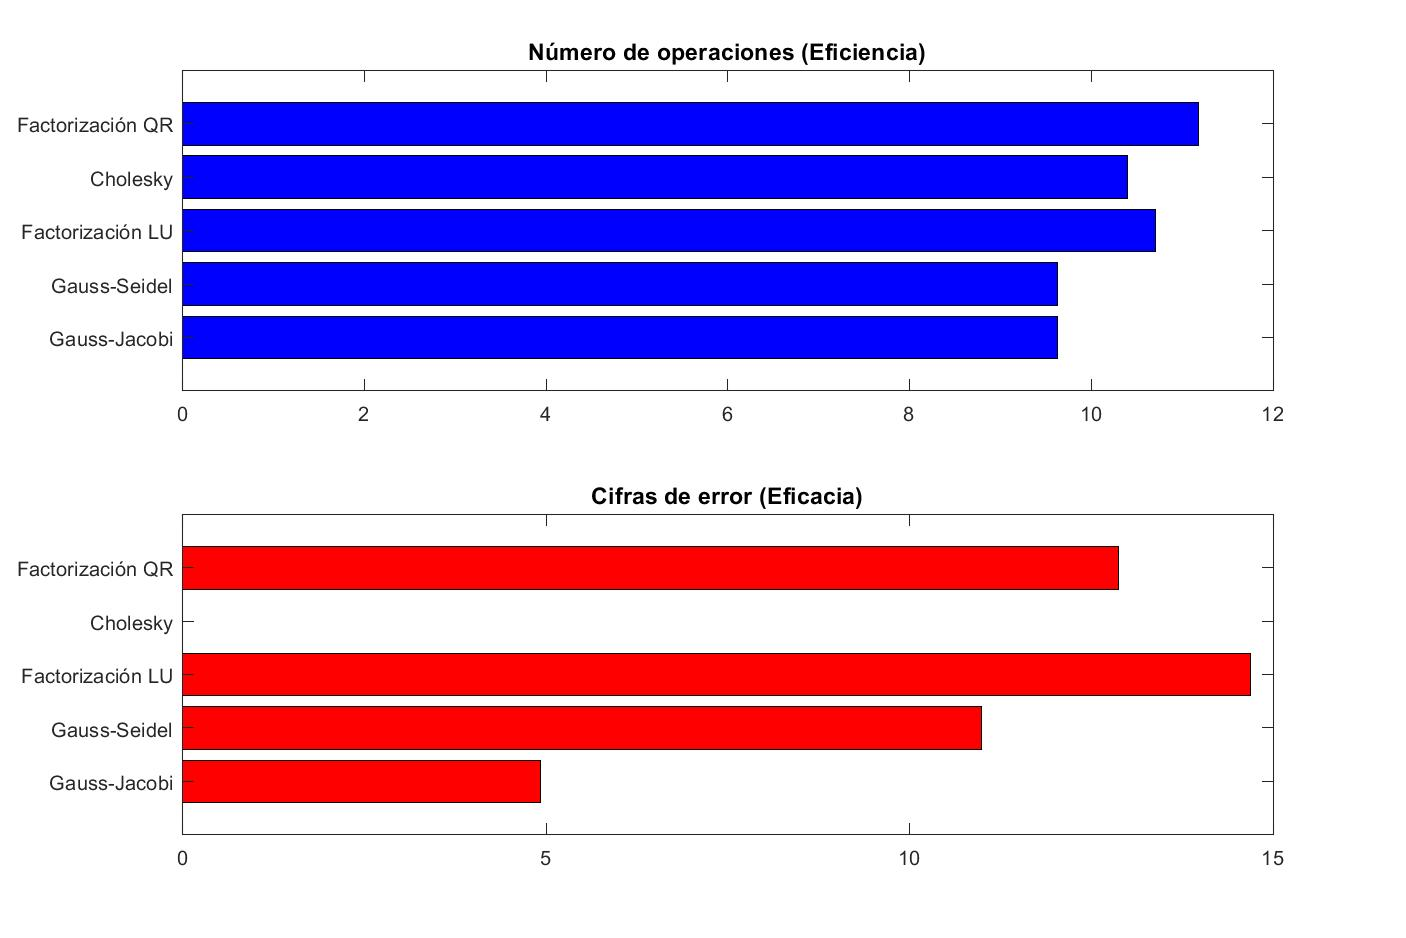
\includegraphics[width=15cm]{imagenes/SE/SE4225.jpg}}

\figura{Ranking Sistema 4225x4225}
{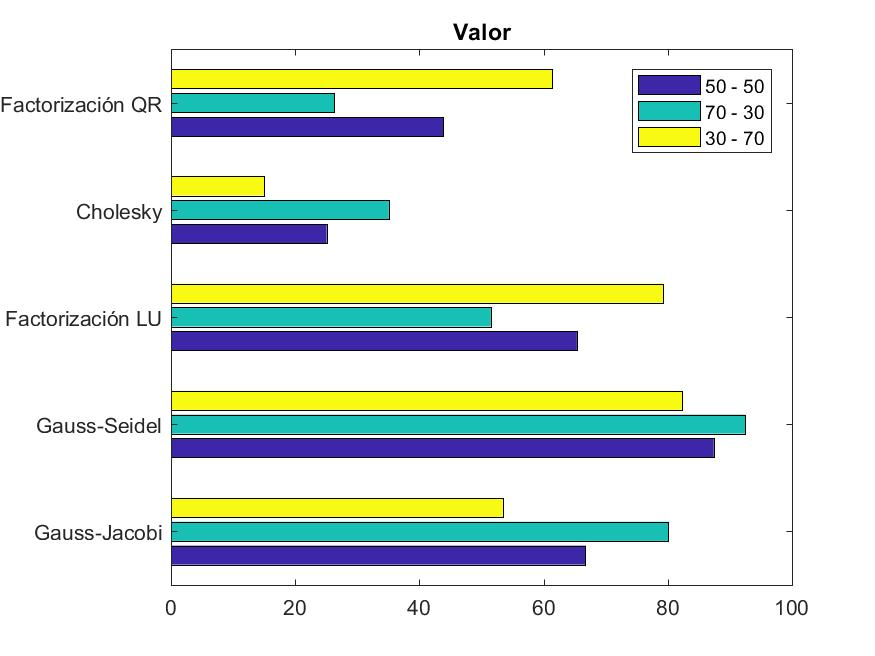
\includegraphics[width=15cm]{imagenes/SE/ranking4225.jpg}}

Como referencia para el error, se utiliza la función $linsolve(A, b)$ que entrega la solución al sistema $Ax = b$ planteado anteriormente. Se debe tener en cuenta que según Matlab, $linsolve$ utiliza el método LU con cuando la matriz es cuadrada. Se presenta la siguiente tabla con la síntesis numérica en cada sistema:

\begin{table}[]
\centering
\begin{tabular}{|c|c|c|}
\hline
\textbf{Método} & \textbf{Error 289x289} & \textbf{Error 1089x1089}\\ \hline
Gauss-Jacobi       &  4.764869937272565e-16    & 3.408631555713930e-15 \\ \hline
Gauss-Seidel      & 4.764869937272565e-16     & 3.408631555713930e-15 \\ \hline
Factorización LU & 3.573652452954423e-16 & 2.606600601428299e-15\\ \hline
Factorización QR & 4.169261195113493e-15 & 1.864721968714091e-14\\ \hline
Cholesky         & 0.640235655559680     & 0.980403097444425\\ \hline
\end{tabular}
\caption{Errores sistema de ecuaciones (1-2)}
    \label{tab:my_label}
\end{table}

\begin{table}[]
\centering
\begin{tabular}{|L|L|}
\hline
\textbf{Método} & \textbf{Error 4225x4225}\\ \hline
Gauss-Jacobi      & 1.209865469601576e-05\\ \hline
Gauss-Seidel      & 1.039802516230656e-11\\ \hline
Factorización LU & 2.071706650854928e-15\\ \hline
Factorización QR & 1.325892256547154e-13\\ \hline
Cholesky        & 0.999987604224092\\ \hline
\end{tabular}
\caption{Errores sistema de ecuaciones (2-2)}
    \label{tab:my_label}
\end{table}

\begin{table}[]
\centering
\begin{tabular}{|c|c|c|c|}
\hline
\textbf{Método} & \textbf{Coste 289x289} & \textbf{Coste 1089x1089} & \textbf{Coste 4225x4225}\\ \hline
Gauss-Jacobi       & 10051998     & 565321680 & 4.229225e+09\\ \hline
Gauss-Seidel      & 2747234     & 143101134 & 4.229225e+09\\ \hline
Factorización LU & 16216368 & 862755168 & 5.030603e+10\\ \hline
Factorización QR & 48358948 & 2.584122948e+09 & 1.508556e+11\\ \hline
Cholesky         & 8129281     & 431674881 & 2.515748e+10\\ \hline
\end{tabular}
\caption{Coste operacional sistema de ecuaciones}
    \label{tab:my_label}
\end{table}


\subseccion{Análisis en sistemas de ecuaciones}

Como se puede observar en las figuras 5-1 a 5-13, los métodos aplicados obtienen soluciones similares y sus variaciones de error son poco perceptibles dado el tamaño de las dimensiones. La excepción a esto es el método de Cholesky, el cual no se logra implementar correctamente, causando que el error aumente según el tamaño del sistema. Teniendo esto en cuenta, el análisis no considera los resultados de éste método ya que no se garantizan resultados correctos.

En cuanto a Gauss-Jacobi, es esperado que el error obtenido siempre sea igual o mayor que Gauss-Seidel, ya que el segundo es una mejora del primero. Seidel va a obtener una convergencia más rápida al resultado ya que utiliza los valores obtenidos en la iteración actual, lo cual está demostrado que tiene menor error que los valores de la iteración anterior, repercutiendo en una reducción significativa del coste operacional. Lo anterior se va acrecentando a medida que aumenta el tamaño del sistema.

Entre todos los métodos, la factorización QR toma más operaciones, y el menor es Seidel. La ventaja de QR es que permite la resolución de sistemas con matrices no cuadradas, a diferencia de las demás.

Se debe notar que para los métodos Gauss-Jacobi y Gauss-Seidel se utiliza un límite de iteraciones a 1000. Ambos se detuvieron en tal valor para el sistema $4225x4225$, mostrando claramente la diferencia de eficacia que existe entre los métodos. Por otro lado, la eficiencia de la factorización LU se mantiene constante, lo cual es un factor importante para la escalabilidad del problema - probablemente la razón principal por la que la función de Matlab $linsolve$ utiliza este método -.

\capitulo{Conclusiones}

\seccion{Conclusiones de funciones no lineales}

A partir de los datos obtenidos en los experimentos del capítulo 4, es claro que la mayoría de los métodos logran converger hacia la solución con una excelente exactitud para la función (1), la excepción siendo Aitken. Otro elemento a destacar es la dependencia que tiene Regula Falsi frente a la estructura de la función. Esto ocurre particularmente cuando trabaja sobre curvas con una pendiente pronunciada, causando una convergencia más lenta que incluso Bisección.

En cuanto a eficiencia y eficacia, los resultados fueron los esperados respecto a Newton-Raphson, mientras que Secante se encuentra a la par con éste. Debe considerarse que ambas tienen mayor inestabilidad que los otros métodos para las primeras iteraciones en la segunda función, pero a pesar de ello resultan ser las más eficaces al disminuir el error a razón cuadrática.

Se puede ver en el experimento la aceleración de convergencia que obtiene el Punto Fijo utilizando Aitken o Steffensen donde sin duda Steffensen llega a ser mejor que Newton-Raphson y Secante, como es el caso con la función (2).

Por otro lado, se puede notar que Newton Multivariable converge al resultado a razón cuadrática. 

Finalmente, no se recomienda el uso de Bisección si se busca valores precisos en poco tiempo ni Regula Falsi si se desea un método de eficiencia confiable (no se sabe cuanto puede tardar). Newton-Raphson es conocida por su efectividad, pero existen otros métodos como Secante y Punto Fijo Steffensen. La contraparte de aplicar Punto Fijo es que se debe hacer un cálculo previo, y se debe considerar los intervalos donde se cumple la condición de convergencia. Gracias a la heurística aplicada, se pueden clasificar los métodos de acuerdo a la importancia que se le den a los criterios de eficiencia y eficacia, puesto que lo principal de aplicar un método antes que otro, es solucionar problemas de acuerdo al contexto donde se aplican.\\

\seccion{Conclusiones de Sistemas de ecuaciones}

Se pueden concluir diversos puntos sobre los experimentos realizados:

\begin{itemize}
    \item No se puede asegurar nada del comportamiento del método Cholesky, ya que no se logra una buena aproximación a la solución. 
    %Por otro lado, tampoco se puede asegurar que el método falla globalmente al usar la norma infinita, que posiblemente detecte un error en particular, evitando que el error tienda a 0.
    \item La factorización LU puede no ser tan eficiente para sistemas pequeños como Gauss-Seidel o Gauss-Jacobi, pero resulta la más eficaz a medida que el problema aumenta de tamaño. 
    \item Factorización QR es la menos eficiente por lo general entre los métodos descritos, pero permite soluciones para problemas que no se pueden implementar en otros métodos.
    \item Gauss-Seidel es siempre mejor que Gauss-Jacobi. Ambos métodos requieren un número de iteraciones proporcional al tamaño del problema para lograr una eficacia determinada.
    \item Es de vital importancia el tipo de matriz con que se esta tratando, si es del tipo triangular se puede aplicar una sustitución progresiva o regresiva para ahorrar un tiempo de cálculo considerable. A su vez, no se puede aplicar cualquier método en cualquier problema. Algunos métodos requieren condiciones para converger correctamente al resultado.
\end{itemize}



% Para sintetizar el desarrollo realizado, se puede indicar que cada uno de los métodos tiene sus ventajas y desventajas, y que dependiendo de lo que se desea solucionar, se debe seleccionar el método adecuado, considerando los factores descritos anteriormente y también el posible gasto computacional que conlleva la aplicación de los métodos en algún lenguaje de programación específico.

% Finalmente, el objetivo del laboratorio fue cumplido, ya que se pudieron implementar los 6 métodos descritos al inicio en MATLAB, lo que ayuda a comprender y manejar la programación en este lenguaje, para así poder contar con esta poderosa herramienta para los siguientes laboratorios de la asignatura, y también para, quizás en el futuro, poder utilizarlo para alguna tarea en el ámbito de la ingeniería informática. Además, con este tipo de actividades prácticas se consolida el aprendizaje realizado en las clases de cátedra, consiguiendo comprender los conceptos de mejor manera, aplicando éstos a la resolución de problemas reales.

%\capitulo{Anexos}

% \seccion{Descripción de los métodos}
% En este capítulo se presenta una breve descripción de cada uno de los métodos, indicando además el procedimiento para aproximar las soluciones a las distintas ecuaciones.

% \subseccion{Método de la Bisección}
% Este es uno de los métodos más sencillos e intuitivos para resolver ecuaciones con una variable. Se basa en el teorema del valor medio que establece que toda función continua $f$ en el intervalo cerrado $[a,c]$ toma todos los valores que se hallan entre $f(a)$ y $f(b)$. Lo que en otras palabras es que todo los valores entre $f(a)$ y $f(b)$ son imagen de al menos un valor del intervalo $[a,b]$. Si $f(a)$ y $f(b)$ tienen signos opuestos, entonces existe, con certeza, un valor $p$ en $[a,b]$ tal que $f(p)=0$. Con esto se asegura la existencia de al menos una solución para la ecuación.

% El método consiste en lo siguiente:
% \begin{enumerate}
% \item Debe existir seguridad acerca de la continuidad de la función $f$ en el intervalo $[a,b]$.
% \item Se debe verificar que $f(a)*f(b)<0$.
% \item Se calcula el punto medio $m$ del intervalo. Si $f(m)=0$, entonces se ha encontrado la raíz de la ecuación.
% \item En caso de que no lo sea, se verifica si $f(m)$ tiene signo opuesto con $f(a)$ o con $f(b)$.
% \item Se redefine el intervalo de trabajo como $[a,m]$ o como $[m,b]$, según se haya determinado en cuál de estos intervalos ocurre un cambio de signo.
% \item Se sigue evaluando con este nuevo intervalo, realizando el mismo procedimiento, hasta alcanzar la precisión deseada.
% \end{enumerate}

% Este método asegura la convergencia si se cumplen las condiciones de continuidad de la función en $[a,b]$ y si $f(a)$ y $f(b)$ tienen signos opuestos. En caso de que exista más de una solución en el intervalo, el método converge pero es complicado saber a qué solución está acercándose.

% Finalmente, este método converge linealmente, por lo que es un poco lento.

% \subseccion{Método del Punto Fijo}
% Este método es un método iterativo que permite determinar las raíces de una función de la forma $f(x)$, siempre y cuando se cumplan los criterios de convergencia.

% El procedimiento se inicia con una estimación de la raíz $x$, que se mejora por cada iteración hasta alcanzar la convergencia.

% El método consiste en lo siguiente:
% \begin{enumerate}
% \item Estimar $x$ tal que $f(x)=0$.
% \item Sumar x en cada lado de la ecuación anterior, obteniendo $f(x)+x=x$, donde $f(x)+x=g(x)=x$.
% \item Se obtiene de $g(x)$ su derivada $g'(x)$.
% \item Se resuelve la desigualdad $-1 \leq g'(x) \leq 1$, donde se obtendrá el rango de valores entre los que se encuentra el punto fijo, llamado $R$.
% \item Con $R$ se busca la raíz en $g(x)$, es decir, $g(R)=R$, haciendo iteración de las operaciones.
% \end{enumerate}

% \subseccion{Método de la Secante}
% El Método de la Secante es un método para encontrar las soluciones de una ecuación de forma iterativa.

% Es una variación del Método de Newton-Rhapson (que se explica más adelante en este mismo capítulo), donde en vez de calcular la derivada en el punto de interés, se aproxima la pendiente a la recta que une a la función evaluada en el punto de interés y el punto de la iteración anterior.

% En otras palabras, este método es un algoritmo de aproximación que usa las raíces de las líneas secantes para aproximar mejor la raíz de la función $f$.

% Para este método, la ecuación de recurrencia es:
% \begin{equation}
% x_{n+1}=x_{n}-\frac{x_{n}-x_{n-1}}{f(x_{n})-f(x_{n-1})} * f(x_{n})
% \end{equation}

% Como se aprecia en la ecuación (2.1), son necesarias dos aproximaciones para iniciar el proceso.

% De manera general, el proceso consiste en:
% \begin{enumerate}
% \item Obtener ecuación de la recta que pasa por $(x_{n-1},f(x_{n-1}))$ y $(x_{n},f(x_{n}))$.
% \item Se selecciona como siguiente elemento de la recurrencia el valor $x_{n+1}$, que es la intersección de la secante con el eje de las abscisas.
% \item Se obtiene el nuevo valor de la fórmula y se repite el proceso hasta el nivel deseado de precisión.
% \end{enumerate}

% \subseccion{Método Regula Falsi}
% Este método, también conocido como el Método de la Falsa Posición, es un método iterativo para encontrar la solución de ecuaciones no lineales. Se caracteriza por combinar el Método de la Bisección y el Método de la Secante.

% Al igual que en el Método de Bisección, se parte con un intervalo inicial $[a_{0},b_{0}]$ con $f(a_{0})$ y $f(b_{0})$ de signos opuestos, lo que garantiza que en ese intervalo se encuentra una de las soluciones buscadas.

% El algoritmo obtiene en cada paso un intervalo más pequeño $[a_{k},b_{k}]$ que sigue incluyendo la raíz de la función $f$.

% Para cada intervalo $[a_{k},b_{k}]$ se calcula un punto interior $c_{k}$ con la fórmula mostrada a continuación.

% \begin{equation}
% c_{k}=\frac{f(b_{k})*a_{k}-f(a_{k})*b_{k}}{f(b_{k})-f(a_{k})}
% \end{equation}

% El proceso para este método es el siguiente:
% \begin{enumerate}
% \item Seleccionar el intervalo inicial $[a_{0},b_{0}]$.
% \item Calcular el punto interior $c_{k}$ con la fórmula (2.2).
% \item Evaluar $f(c_{k})$. Si es suficientemente pequeño, $c_{k}$ es la raíz buscada.
% \item Si no, el próximo intervalo $[a_{k+1},b_{k+1}]$ será:
% \begin{enumerate}
% \item $[a_{k},c_{k}]$ si $f(a_{k})$ y $f(c_{k})$ tienen signos opuestos.
% \item $[c_{k},b_{k}]$ en caso contrario.
% \end{enumerate}
% \end{enumerate}

% \subseccion{Método de Newton-Raphson}
% Es un método eficiente para encontrar aproximaciones de las raíces de una función real.

% Este método es un método abierto, lo que quiere decir que no está asegurada su convergencia global. La única forma de alcanzar la convergencia es seleccionar un valor suficientemente cercano a la raíz buscada. Es importante que este método tiene dificultades cuando la función tiene pendientes grandes o múltiples puntos de inflexión cerca de la raíz, lo que trae como consecuencia un aumento de probabilidad de que no exista convergencia.

% La fórmula de iteración para este método es la siguiente.

% \begin{equation}
% x_{n+1}=x_{n}-\frac{f(x_{n})}{f'(x_{n})}
% \end{equation}

% Donde se va calculando los números siguientes con la ecuación (2.3) hasta tener la precisión deseada.

% \subseccion{Método de Newton-Raphson de segundo orden}
% El método de Newton-Raphson de segundo orden es igual al método de Newton-Raphson, sólo que ahora se considera la segunda derivada de la función.

% La fórmula de iteración para este método es la siguiente.

% \begin{equation}
% x^{+}_{n+1} = x_{n}-\frac{f'(x_{n})}{f''(x_{n})}+\frac{\sqrt{[f'(x_{n})]^{2}-2*f''(x_{n})*f(x_{n})}}{f''(x_{n})}
% \end{equation}

% \begin{equation}
% x^{-}_{n+1} = x_{n}-\frac{f'(x_{n})}{f''(x_{n})}-\frac{\sqrt{[f'(x_{n})]^{2}-2*f''(x_{n})*f(x_{n})}}{f''(x_{n})}
% \end{equation}

% Donde se selecciona el valor de la ecuación (2.4) o (2.5) evaluando el punto en la función. En otras palabras, se evalúa $f(x^{+}_{n+1})$ y $f(x^{-}_{n+1})$ y se selecciona la más cercana a cero.

\end{document}